%-------------------------------------------------------------------------------
% This file provides a skeleton ATLAS note.
% \pdfinclusioncopyfonts=1
% This command may be needed in order to get \ell in PDF plots to appear. Found in
% https://tex.stackexchange.com/questions/322010/pdflatex-glyph-undefined-symbols-disappear-from-included-pdf
%-------------------------------------------------------------------------------
% Specify where ATLAS LaTeX style files can be found.
\newcommand*{\ATLASLATEXPATH}{latex/}
% Use this variant if the files are in a central location, e.g. $HOME/texmf.
% \newcommand*{\ATLASLATEXPATH}{}
%-------------------------------------------------------------------------------
\documentclass[NOTE, atlasdraft=true, texlive=2016, UKenglish]{\ATLASLATEXPATH atlasdoc}
% The language of the document must be set: usually UKenglish or USenglish.
% british and american also work!
% Commonly used options:
%  atlasdraft=true|false This document is an ATLAS draft.
%  texlive=YYYY          Specify TeX Live version (2016 is default).
%  coverpage             Create ATLAS draft cover page for collaboration circulation.
%                        See atlas-draft-cover.tex for a list of variables that should be defined.
%  cernpreprint          Create front page for a CERN preprint.
%                        See atlas-preprint-cover.tex for a list of variables that should be defined.
%  NOTE                  The document is an ATLAS note (draft).
%  PAPER                 The document is an ATLAS paper (draft).
%  CONF                  The document is a CONF note (draft).
%  PUB                   The document is a PUB note (draft).
%  BOOK                  The document is of book form, like an LOI or TDR (draft)
%  txfonts=true|false    Use txfonts rather than the default newtx
%  paper=a4|letter       Set paper size to A4 (default) or letter.

%-------------------------------------------------------------------------------
% Extra packages:
%\usepackage[backend=biber, subfigure, full]{\ATLASLATEXPATH atlaspackage}
\usepackage{\ATLASLATEXPATH atlaspackage}
% Commonly used options:
%  biblatex=true|false   Use biblatex (default) or bibtex for the bibliography.
%  backend=bibtex        Use the bibtex backend rather than biber.
%  subfigure|subfig|subcaption  to use one of these packages for figures in figures.
%  minimal               Minimal set of packages.
%  default               Standard set of packages.
%  full                  Full set of packages.
%-------------------------------------------------------------------------------
% Style file with biblatex options for ATLAS documents.
\usepackage{\ATLASLATEXPATH atlasbiblatex}
% Commonly used options:
%  backref=true|false    Turn on or off back references in the bibliography.

% Package for creating list of authors and contributors to the analysis.
\usepackage{\ATLASLATEXPATH atlascontribute}

% Useful macros
\usepackage{\ATLASLATEXPATH atlasphysics}
\usepackage{amsmath}
\usepackage{lscape}
\usepackage{verbatim}
\usepackage{graphicx}
\usepackage{float}
\usepackage{subfig}
\usepackage{booktabs}
% See doc/atlas_physics.pdf for a list of the defined symbols.
% Default options are:
%   true:  journal, misc, particle, unit, xref
%   false: BSM, heppparticle, hepprocess, hion, jetetmiss, math, process,
%          other, snippets, texmf
% See the package for details on the options.
%\usepackage[output=true]{\ATLASLATEXPATH atlastodo}

% Files with references for use with biblatex.
% Note that biber gives an error if it finds empty bib files.
% \addbibresource{ANA-HIGG-2020-08-INT1.bib}
\addbibresource{bib/ATLAS.bib}
\addbibresource{bib/CMS.bib}
\addbibresource{bib/ConfNotes.bib}
\addbibresource{bib/PubNotes.bib}

% Paths for figures - do not forget the / at the end of the directory name.
\graphicspath{{logos/}{figures/}}

% Add you own definitions here (file ANA-HIGG-2020-08-INT1-defs.sty).
\usepackage{ANA-HIGG-2020-08-INT1-defs}
%-------------------------------------------------------------------------------
% Generic document information
%-------------------------------------------------------------------------------

% Title, abstract and document 
\input{ANA-HIGG-2020-08-INT1-metadata}
% Author and title for the PDF file
\hypersetup{pdftitle={ATLAS document},pdfauthor={The ATLAS Collaboration}}

%-------------------------------------------------------------------------------
% Content
%-------------------------------------------------------------------------------
\begin{document}

\maketitle

\tableofcontents

% List of contributors - print here or after the Bibliography.
%\PrintAtlasContribute{0.30}
\clearpage

\section{Introduction}
\label{sec:intro}


\paragraph{}The discovery of Higgs boson by ATLAS and CMS experiment in 2012 opens a new era for particle physics, and provides a new opportunity to search for new physics beyond Standard Model, such as the new source of CP-violation required by the observed baryon asymmetry in the universe. In the Standard Model the expected Higgs boson is a scalar boson with $J^{pc} = 0{++}$, till now all the experimental results in ATLAS and CMS are consistent with this prediction within the uncertainty.  However, limited by the statistics, the direct Higgs CP measurements are performed only in very recent period  \cite{VBFHtautau}\cite{ttHyy}\cite{CMS_VBFHtautau}\cite{CMS_ttHyy}. All of these observations show no derivation from SM, but the restriction is not so satisfying. 


\paragraph{} The focus of this work is the CP property of Higgs boson in its interaction with gauge vector bosons. The test is performed through the largest HVV production mode in LHC, Vector Boson Fusion, in diphoton decay channel, with 140 $fb^{-1}$ p-p collision data collected by ATLAS detector at $\sqrt(s)=13TeV$ during 2015 to 2018. In order to have a more sensitive result and be independent with CP-even observables, the Optimal Observable is introduced as in previous di-tau channel analysis. 



\paragraph{}The Effective Field Theory and Optimal Observable are introduced in Sec.~\ref{sec:theory}. Sec.~\ref{sec:atlasdet} and Sec.~\ref{sec:dataMC} show a brief description about ATLAS detector and the simulated data we used in this analysis. In Sec.~\ref{sec:sel} and Sec.~\ref{sec:model}, we presented the main analyses procedure, including the event selection, categorization and event modelling. Following in Sec.~\ref{sec:syst} is the experimental uncertainty considered, and statistic model constructed for parameters estimation is in Sec ~\ref{sec:fit}. The results and conclusions are discussed in Sec.~\ref{sec:result} and Sec.~\ref{sec:conclusion}.  


\clearpage
\section{Theoretical framework}
\label{sec:theory}
\paragraph{}\todo{introduce what the the EFT Lagrangian is, before speaking of Htau combination} The effective Lagrangian is the SM Lagrangian augmented with CP-odd operator of mass dimension 6, involving the Higgs field and electroweak gauge fields. The other interactions between Higgs/vector boson and fermions/gluons are assumed to be the same with SM prediction. The Lagrangian is be written as: 

\begin{center}
\begin{math}
\mathcal{L}_{eff} = \mathcal{L}_{SM}+ \tilde{g}_{HAA}H\tilde{A}_{\mu\nu}A^{\mu\nu} + \tilde{g}_{HAZ}H\tilde{A}_{\mu\nu}Z^{\mu\nu} + \tilde{g}_{HZZ}H\tilde{Z}_{\mu\nu}Z^{\mu\nu} + \tilde{g}_{HWW}H\tilde{W}_{\mu\nu}^{+}W^{-\mu\nu}
\end{math}
\end{center}
\todo{Please add citation to the original EFT papers where this Lagrangian is from, say that this is *after* symmetry breaking! and cite }
Where $V^{\mu\nu}$ and $\tilde{V}^{\mu\nu}=\epsilon^{\mu\nu\rho\sigma}V_{\rho\sigma} $ (with $V=W^{\pm},Z,A$) denotes the vector field strength. Among the 4 coupling constants $g_{HVV}$ only 2 of them are independent due to the U(1)*SU(2) \todo{use latex math!} constrains, they can be written into two dimensionless coupling $\tilde{d}$ and $\tilde{d}_B$ \todo{use latex equation to cite them, also detail who theses couplings relate to tilde-d before}. As the different contribution from various vector electroweak gauge boson fusion process could not be distinguished experimentally, an arbitrary choice $\tilde{d}$ = $\tilde{d}_B$ is adopted. So the following relation could be derived: 

\begin{center}
\begin{math}
\tilde{g}_{HAA} = \tilde{g}_{HZZ} = \frac{1}{2} \tilde{g}_{HWW} = \frac{g}{2m_{W}}\tilde{d} \qquad and \qquad \tilde{g}_{HAZ}=0
\end{math}
\end{center}

The parameter $\tilde{d}$ becomes the only one describing the CP violation in VBF Higgs production. \todo{add Lorentz sturcture of the vertices and explain the different term}.The corresponding matrix element could be written as the sum of a CP-even SM contribution $\mathcal{M}_{SM}$ and a CP-odd contribution $\mathcal{M}_{CP-odd}$ from EFT, and $\tilde{d}$ could be factorized out\todo{refer back to the equation mentioning the Lorentz structure of the vertices to justify this statement}:

\begin{center}
\begin{math}
\mathcal{M}=\mathcal{M}_{SM}+\tilde{d}\cdot\mathcal{M}_{CP-odd} 
\end{math}
\end{center}

The VBF cross section is proportional to the squared matrix element: 

\begin{center}
\begin{math}
|\mathcal{M}|^2 = |\mathcal{M}_{SM}|^2 + \tilde{d}\cdot2 Re(\mathcal{M}^{\ast}_{SM} \mathcal{M}_{CP-odd}) + \tilde{d}^2\cdot|\mathcal{M}_{CP-odd}|^2
\end{math}
\end{center}

The first term and last term are both CP-even, only the second term from the interference of 2\todo{two not 2, every where in the text, numbers should be written as words} matrix element is CP-odd, representing a new source of CPV in Higgs field. This CP-odd term would vanish after integrated after a CP-symmetric phase space, so it does not contribute to the total cross section and observed event yields after applying CP-symmetric selection criteria. The third term could increase the total cross section by an amount of $\tilde{d}^2$. 

%why comment?
\todo{add all the removed details!}
\begin{comment}
\paragraph{}In the decay mode the EFT operator brings new source for Higgs decay to di-photon final state. At tree level these effective operators will contribute to the partial decay width of Higgs boson in $H\to\gam\gam$, $H\to\gam Z$, $H\to ZZ$ and $H\to WW$ channels. The helicity configuration of the particles in the final state is orthogonal to the SM case, so the interference term is zero. The angular distribution for the final state photon would not be influenced so only the change in number of branching ratio is considered: 

\begin{equation} why ?

\label{eq:Bryy}
\small
\begin{aligned}
Br(H\to\gam\gam) &= \frac{\Gamma(H\to\gam\gam)_{SM}+\delta\Gamma(H\to\gam\gam)}{\Gamma(H)_{SM}+\delta\Gamma(H\to\gam\gam)+\delta\Gamma(H\to\gam Z) + \delta\Gamma(H\to Z^{\ast}Z) + \delta\Gamma(H\to W^{\ast}W)} \\
 & = \frac{0.227\% \times 4.066MeV + 155.425MeV \tilde{g}_{HAA}^2} { 4.088MeV+155.425MeV \tilde{g}_{HAA}^2+7.957MeV \tilde{g}_{HAZ}^2 + 0.00065MeV \tilde{g}_{HZZ}^2 + 0.0036MeV \tilde{g}_{HWW}^2 } 
\end{aligned}
\end{equation}

The numerical contribution from the branching ratio is significant compared with the SM prediction, only using the event yield can already provide a strict constraint on the CPV in this model. However, considering the cross section could be influenced by other CP-conserving new physics, event yields are unconstrained in the main part of this analysis.

\begin{figure}[h]
   \centering
   \includegraphics[width=.7\textwidth]{figure/BrHyy.png}
   \caption{Higgs to di-photon branching ratio as a function of CP mixing parameter $\tilde{d}$. }
   \label{fig:BrHyy}
\end{figure}
\end{comment}

\todo{describe first that typically people used signed dphijj and cite the Zeppenfeld CP paper similar to Htau INT, then introduce that the OO is more optimal}
\paragraph{}The VBF Higgs decay final state contains the reconstructed Higgs boson and two tagging jets from VBF topology. This can be characterized in a seven-dimension phase space, when fixing the Higgs mass, neglecting jet masses and exploiting the transverse momentum conservation. The Optimal Observable combines the information from total phase space into one single variable, so it shows much better performance than traditional operators. It is defined as the ratio of the interface term in the matrix element to the SM contribution: 

\begin{center}
\begin{math}
\mathcal{OO} = \frac{2Re(\mathcal{M}^{\ast}_{SM} \mathcal{M}_{CP-odd})}{|\mathcal{M}_{SM}|^2}
\end{math}
\end{center}


\paragraph{}The Optimal Observable is a CP-odd variable, so it can be a probe of CPV in the HVV vertex. In the SM the expectation\todo{mean value} value would vanish(<OO>=0), so any non-zero mean value or asymmetry in distribution of Optimal Observable indicates the physics beyond SM, either stemming from CPV, or originating from rescattering effects ~\cite{Brehmer_2018} \todo{detail this }. Plot ~\ref{fig:OOwithd} shows the distribution of Optimal Observable for several $\tilde{d}$ VBF signal model, with obvious non-zero mean value and asymmetry shape. 

\todo{plot is very low resolution, use the original pdf or ebs file and not png}
\begin{figure}[h]
	\centering
	\includegraphics[width=.7\textwidth]{figure/OOind.png}
	\caption{Optimal Observable distribution in VBF process, with $\tilde{d}=-0.02$, $\tilde{d}=0$ (SM) and $\tilde{d}=0.02$}
	\label{fig:OOwithd}
\end{figure}

\paragraph{}\todo{Mention first (and cite the OO equation) that to measure OO one needs to measure the 7 phase space variables needed to characterize the event then speak of Hawk} The package HAWK ~\cite{HAWK_2015} provides a calculation for VBF and VH process matrix element, with the kinematic variables in final state (4-momenta of the Higgs boson and 2 tagging jets in VBF). For the initial state, the momentum fraction Bjorken $x_1$($x_2$) \todo{say that 1 and 2 are incoming and outgoing partons} of parton can be derived by energy-momentum conservation: 

\begin{center}
\begin{math}
x_{1,2}^{reco}=\frac{m_{Hjj}}{\sqrt{s}}e^{\pm y_{Hjj}}
\end{math}
\end{center}

Where $m_{Hjj}$ and $y_{Hjj}$ are the invariant mass and pseudo rapidity of Higgs+2 tagging jets system. The matrix element calculation performs a summation of all possible flavor configurations in initial and final state ij->klH weighted by CT10 leading order parton distribution functions(PDFs.) \todo{speak first that it's weighted a parton distribution function and then mention CT10 in the next section, say also that the shape doesn't depend on PDF choice and say how these parameters are estimated at truth and reco level}. 

\begin{center}
\begin{math}
2Re(\mathcal{M}^{\ast}_{SM}\mathcal{M}_{CP-odd}) = \sum_{i,j,k,l} f_i(x_1)f_j(x_2)2Re((\mathcal{M}_{SM}^{ij \to klH})^{\ast} \mathcal{M}_{CP-odd}^{ij\to klH} ) 
\end{math}
\\
\begin{math}
|\mathcal{M}_{SM}|^2 = \sum_{i,j,k,l} f_i(x_1)f_j(x_2)|\mathcal{M}_{SM}^{ij \to klH}|^2
\end{math}
\end{center}





%\clearpage
\section{ATLAS Detector}
\label{sec:atlasdet}
\paragraph{} The ATLAS detector is one of two general detectors at LHC. It is normally forward-backward symmetric and covers nearly all the solid angle around proton-proton interaction point. From inner it consists of an inner tracker detector(ID), a superconducting solenoid, electromagnetic and hadronic calorimeter, and a muon spectrometer. 3 main component of Inner Detector, pixel detector, semiconductor tracker and transition radiation tracker provide precise measurement of transverse momentum, direction, charge for the charged particle, as well as a preliminary identification to b-jets in barrel region $(|\eta|<2.5)$. The whole Inner Detector is immersed in a 2T axial magnetic field provided by the solenoid. The outer part, electromagnetic calorimeter is a high granularity lead/liquid-argon(LAr) sampling calorimeter, measures the electromagnetic shower in barrel $(|\eta|<1.475)$ and endcap $(1.375<|\eta|<3.2)$ regions. Following hadronic calorimeter can reconstruct the hadronic shower with steel and scintillator tiles $(|\eta|<1.7)$, copper/LAr $(1.5<|\eta|<2.7)$ or copper-tungsten/LAr $(3.1<|\eta|<4.9)$ respectively. The outermost layer muon spectrometer comprises 3 large superconducting eight-coil toroids, separate trigger chambers $(|\eta|<2.4)$ and precision tracking chambers $(|\eta|<2.7)$.

\paragraph{} The ATLAS data-taking system uses a two-level system: a hardware-based level trigger(L1) to reduce the event rate to at most 100 kHz, and a software-based level trigger(L2) to reduce the event rate to approximately 1 kHz. 


\clearpage
\section{Data and Monte Carlo Samples}
\label{sec:dataMC}

\paragraph{} This analysis uses LHC proton-proton collision data collected by ATLAS detector from 2015 to 2018, at central-of-mass energy $\sqrt(s)=13TeV$. After requiring good data quality the data set amounts to integrated luminosity 139.8 $fb^{-1}$. The mean number of interactions per bunch crossing, $\mu$, was 34 on average, varying from $24$ in 2015-2016 to $37$ in 2018 data. Events were selected by a di-photon trigger with pT thresholds of 35GeV and 25 GeV for leading and sub-leading photon. A tight photon identification and isolation requirement are applied. On average the trigger efficiency can reach to 98\% after the event selection. 

\begin{table}[htbp]
\centering
\begin{tabular}{l|c}
\hline
Period & $\int \mathcal{L} dt [fb^{-1}]$ \\ \hline
2015   & 3.2                   \\
2016   & 32.9                  \\
2017   & 43.8                  \\
2018   & 59.9                  \\ \hline
total  & 139.8                 \\
\hline
\end{tabular}
\caption{Integrated luminosity in ATLAS RunII period. The combined luminosity uncertainty is 1.7\% [ref:Run2Lumi]}
\label{tab:dataLumi}
\end{table}

\paragraph{} The main Standard Model processes considered in this work are gluon-fusion (ggF) Higgs production, Vector Boson Fusion (VBF) Higgs production, and continuum diphoton production. For the ggF and VBF process, Monte-Carlo (MC) generator provides a precise simulation, the detailed generator, parton distribution functions (PDFs) and perturbative order in QCD is summarized in Table ~\ref{tab:MC}. 

\begin{center}
\centering
\begin{table}[htbp]
\begin{tabular}{l|l|l|l|l|l}
\hline
Process        & Generator & Showering & PDF sets  & QCD order         & $\sigma [pb] \sqrt{s}=13TeV$ \\
\hline
VBF            & Powheg    & PYTHIA8   & PDF4LHC15 & NNLO(QCD)+NLO(EW) & 3.75                         \\
ggF            & Powheg    & PYTHIA8   & PDF4LHC15 & NNLO(QCD)+NLO(EW) & 28.3                         \\
$\gamma\gamma$ & Sherpa    & Sherpa    & CT10      &                   &                             	\\
\hline
\end{tabular}
\caption{Monte Carlo samples used in this analysis.}
\label{tab:MC}
\end{table}
\end{center}

\paragraph{}The complicated final state in di-photon + multi-jets process makes it hard to simulate in MC. The Optimal Observable combines the information from 7-dimension phase space, any mismodelling would lead to an biased estimation in OO. So sideband data becomes the best candidate for the background, for both the modelling and event yield. While restricted by the statistics, di-photon continuum background modelling could not be performed by sideband data, so a set of di-photon+jets process MC are generated by Sherpa, with proper hadronization and reconstruction. 

\paragraph{}To simulate the CP violation phenomenon in HVV vertex, a matrix element based reweighting method is performed in the SM VBF sample. The weight is defined by the square of matrix element value of VBF process associated with a specific amount of CP mixing $\tilde(d)$ to the one obtained from SM. The corresponding 2 matrix elements are calculated by HAWK with initial and final state information in each event, assuming a $2\to2+H$ or $2\to3+H$ process. For convenience the weight is parameterized as a function of $\tilde(d)$, so the CPV process in any mixing level could be simulated immediately. 

\begin{center}
\begin{math}
w = 1+\tilde{d}w_1 + \tilde{d}^2w_2
\end{math}
\end{center}

\paragraph{} For all MC generated samples, a full simulation of ATLAS detector response with Geant4 program is performed, except the CPV VBF Higgs process is reweighted from reconstructed SM VBF process. Additional proton-proton interactions (pile-up) are produced using Pythia8 with A2 parameter set and MSTW2008LO PDF set. They are included in the simulation for all generated events such that the distribution of the mean number of interactions per bunch crossing reproduces that observed in the data.


\clearpage
%%\section{Event selection and categorization}
\label{sec:sel}

The VBF candidates in this analysis are selected with the similar methods as other ATLAS measurement of $H\to\gamma\gamma$ in $\sqrt(s)=13TeV$. The simulated samples and data token from detector first go through a preselection stage which imposes requirements on the trigger, the data should have additional data quality checks. Individual objects are then reconstructed and identified as various physical particles, with selection cuts applied to reject background. A final VBF event selection inherited from Simplified Template cross section (STXS) framework is applied for higher VBF event purity. All the following selections are applied in data and SM simulation templates, while the CP-violation effects are estimated with the reweighting method introduced in Sec.~\ref{sec:dataMC}. In this case no selection efficiency for CPV samples is performed here. 

\subsection{Event preselection}
\label{subsec:presel}

\begin{description}
\item{\textbf{Trigger}} \\
2015+2016: The \emph{HLT\_g35\_loose\_g25\_loose} diphoton trigger is used which requires at least 2 reconstructed photons with $E_{T}$ larger 35 and 25 GeV passing loose identification requirements based on the energy leakage in the hadronic compartment and the shower shape in the second layer of the electromagnetic calorimeter. The trigger efficiency, studied in-situ using a bootstrap method, is measured to be $98^{+0.28}_{-0.52}(stat)^{+0.45}_{-0.45}(syst)\%$ [ref:HGamPerf2018]

2017+2018: The \emph{HLT\_g35\_medium\_g25\_medium\_L12EM20VH} diphoton trigger is used, which requires two photon candidates passing medium identification comparing with trigger requirement in 2015+2016. The trigger efficiency is \textcolor{red}{TODO}. 

\item{\textbf{Good run list}} \\
Events must belong to the luminosity blocks specified in: \\
\verb|data15_13TeV.periodAllYear_DetStatus-v89-pro21-02_Unknown_PHYS_StandardGRL_All_Good_25ns.xml| or \\
\verb|data16_13TeV.periodAllYear_DetStatus-v89-pro21-01_DQDefects-00-02-04_PHYS_StandardGRL_All_Good_25ns.xml| or \\
\verb|data17_13TeV.periodAllYear_DetStatus-v99-pro22-01_Unknown_PHYS_StandardGRL_All_Good_25ns_Triggerno17e33prim.xml| or \\
\verb|data18_13TeV.periodAllYear_DetStatus-v102-pro22-04_Unknown_PHYS_StandardGRL_All_Good_25ns_Triggerno17e33prim.xml| \\
These ensure that all the subdetectors relevant for this analysis are fully operative. 

\item{\textbf{Event quality}} \\
The events with data integrity errors in the calorimeter and incomplete events where some detector information is missing are rejected. 

\item{\textbf{Primary vertex}} \\
The event should have at least one reconstructed primary vertex.

\end{description}


\subsection{Object reconstruction and selection}
\label{subsec:objrecon}

This section describe how objects are selected in data and reconstructed simulation samples. Details about the reconstruction are described in [ref:HGamPerf]. 
\begin{description}

\item{\textbf{Photon}} \\
Photons are reconstructed with the clusters in electromagnetic and hadronic calorimeter. Kinematic requirements of $p_{T}>25GeV$ and $|\eta|<2.37$ are applied, as well as a rejection of the crack region between barrel and endcap part $1.37<|\eta|<1.52$. Photon energy is calibrated using latest run-2 calibration corrections for energy scale and resolution, detailed in [ref:EgammaCali]. Also they should be tagged as loose photons at this stage in a shower shape based identification. 

\item{\textbf{Diphoton system}} \\
The two highest $p_{T}$ selected photons are assumed to be the $H\to\gamma\gamma$ candidate. These two photons are used to redefine the primary vertex with a neutral network method[ref:NNPV]. The photon momentum are then corrected with the primary vertex so that they point to the correct vertex. The Higgs candidate photons should furthermore satisfy tight shower shape requirement, as well as track and calorimeter isolation criteria: $ptcone20<0.05\times p_{T}$, $topoetcone20<0.065\times p_{T}$, using a cone of $\Delta R = 0.20$. 

\item{\textbf{Jets}} \\
The jets are reconstructed using the anti-kt algorithm[ref:antikt] with the distance parameter $R=0.4$. and required to have $|\eta|<4.4, p_{T}>30GeV$. An extra medium Jet Vertex Tag (JVT) requirement is applied to suppress the jets coming from pileup. The jet energy scale is corrected using the latest JetEtMissing recommendations. 

\end{description}


\subsection{Selections}
\label{subsec:evtsel}

\begin{description}
\item{\textbf{Kinematic cuts}} \\
All events must contain a diphoton system with invariant mass $m_{\gamma\gamma}\in[105, 160]GeV$. The leading(sub-leading) photons must satisfy a relative $p_{T}$ cut: $p_{T}/m_{\gamma\gamma}>0.35(0.25)$. 
The VBF process requires there must be at least 2 selected jets in each event. Among them 2 jets with highest $p_{T}$ are regarded as VBF jets. In order to focus on VBF events, these two VBF jets should have large pseudo-rapidity separation $|\Delta\eta_{jj}|>2$, large invariant mass $m_{jj}>400GeV$ and satisfy a Zeppenfield $\eta$ cut $|\eta_{\gamma\gamma}-0.5(\eta_{j1}+\eta_{j2})|<5$. 

\item{\textbf{VBF-enriched categories}} \textcolor{red}{NEED VARIFICATION} \\
In Simplified Template cross section(STXS) framework, the VBF production process is encompassed in $qq\to Hqq$ final state category, requiring at least 2 jets in the final state. In addition, events are split into 2 regions based on the transvers momentum of vector sum of momenta of the reconstructed Higgs boson and two leading jet $p_T^{Hjj}>25GeV$ and $p_T^{Hjj}<25GeV$. In each region a gradient Boost Decision Trees (BDTG) is applied to separate VBF from other process. Four exclusive categories are then defined with “tight” and “loose” requirement on the BDT classifier on two $ p_T^{Hjj}$ regions: “$VBF high- p_T^{Hjj} BDT tight$”, “$VBF high- p_T^{Hjj} BDT loose$”, “$VBF low- p_T^{Hjj} BDT tight$”, “$VBF low- p_T^{Hjj} BDT loose$”. Among them “$VBF low- p_T^{Hjj} BDT tight$” category has best VBF signal sensitivity. In this analysis these 4 categories are merged together to ensure the enough statistics. 
\end{description}

\begin{table}[htbp]
\begin{center}
\begin{tabular}{l|cccccc}
\hline
                     & \multicolumn{2}{c}{mc16a}  & \multicolumn{2}{c}{mc16d}  & \multicolumn{2}{c}{mc16e}  \\
                     & VBF yield & selection eff. & VBF yield & selection eff. & VBF yield & selection eff. \\ \hline
initial sumW         & 311.06    &                & 380.07    &                & 514.14    &                \\
GRL                  & 311.06    & 100.00\%       & 380.07    & 100.00\%       & 514.14    & 100.00\%       \\
trigger              & 208.68    & 67.09\%        & 253.66    & 66.74\%        & 343.28    & 66.77\%        \\
DQ                   & 208.68    & 67.09\%        & 253.66    & 66.74\%        & 343.28    & 66.77\%        \\
PV                   & 208.68    & 67.09\%        & 253.66    & 66.74\%        & 343.28    & 66.77\%        \\
2 loose photon       & 172.88    & 55.58\%        & 208.16    & 54.77\%        & 281.25    & 54.70\%        \\
$e-\gamma$ ambiguity & 172.55    & 55.47\%        & 208.16    & 54.77\%        & 281.25    & 54.70\%        \\
trigger match        & 165.28    & 53.13\%        & 184.90    & 48.65\%        & 250.18    & 48.66\%        \\
tightID              & 141.75    & 45.57\%        & 166.46    & 43.80\%        & 225.84    & 43.93\%        \\
isolation            & 129.05    & 41.49\%        & 146.78    & 38.62\%        & 200.67    & 39.03\%        \\
rel. $p_{T}$         & 116.85    & 37.57\%        & 134.22    & 35.31\%        & 183.36    & 35.66\%        \\
mass window          & 116.71    & 37.52\%        & 134.05    & 35.27\%        & 183.12    & 35.62\%        \\
$N_{j}\le2$          & 63.9216   & 20.55\%        & 76.08     & 20.02\%        & 103.19    & 20.07\%        \\
$m_{jj}>400GeV$      & 42.2015   & 13.57\%        & 49.36     & 12.99\%        & 67.18     & 13.07\%        \\
$|\Delta\eta|>2$     & 41.9691   & 13.49\%        & 49.09     & 12.92\%        & 66.80     & 12.99\%        \\
$|\eta^{zepp}|<5$    & 41.9513   & 13.49\%        & 49.07     & 12.91\%        & 66.77     & 12.99\%        \\
VBF cate.            & 36.4902   & 11.73\%        & 42.57     & 11.20\%        & 57.97     & 11.28\%       	\\
\hline
\end{tabular}
\caption{VBF process yields and efficiency in each period from MC.}
\label{tab:cutflowVBF}
\end{center}
\end{table}

\begin{table}[htbp]
\begin{center}
\begin{tabular}{l|cccccc}
\hline
                     & \multicolumn{2}{c}{mc16a}  & \multicolumn{2}{c}{mc16d}  & \multicolumn{2}{c}{mc16e}  \\
                     & ggH yield & selection eff. & ggH yield & selection eff. & ggH yield & selection eff. \\ \hline
initial sumW         & 3994.01   &                & 4879.97   &                & 6601.46   &                \\
GRL                  & 3994.01   & 100.00\%       & 4879.97   & 100.00\%       & 6601.46   & 100.00\%       \\
trigger              & 2589.80   & 64.84\%        & 3147.78   & 64.50\%        & 4261.54   & 64.55\%        \\
DQ                   & 2589.80   & 64.84\%        & 3147.78   & 64.50\%        & 4261.54   & 64.55\%        \\
PV                   & 2589.80   & 64.84\%        & 3147.78   & 64.50\%        & 4261.54   & 64.55\%        \\
2 loose photon       & 2157.52   & 54.02\%        & 2597.77   & 53.23\%        & 3511.85   & 53.20\%        \\
$e-\gamma$ ambiguity & 2153.05   & 53.91\%        & 2597.77   & 53.23\%        & 3511.85   & 53.20\%        \\
trigger match        & 2077.83   & 52.02\%        & 2341.04   & 47.97\%        & 3170.15   & 48.02\%        \\
tightID              & 1787.35   & 44.75\%        & 2098.54   & 43.00\%        & 2849.39   & 43.16\%        \\
isolation            & 1607.01   & 40.24\%        & 1822.68   & 37.35\%        & 2498.35   & 37.85\%        \\
rel. $p_{T}$         & 1489.74   & 37.30\%        & 1702.54   & 34.89\%        & 2330.57   & 35.30\%        \\
mass window          & 1489.39   & 37.29\%        & 1702.15   & 34.88\%        & 2329.97   & 35.29\%        \\
$N_{j}\le2$          & 190.716   & 4.78\%         & 256.13    & 5.25\%         & 342.09    & 5.18\%         \\
$m_{jj}>400GeV$      & 32.8125   & 0.82\%         & 47.39     & 0.97\%         & 62.33     & 0.94\%         \\
$|\Delta\eta|>2$     & 31.1126   & 0.78\%         & 45.31     & 0.93\%         & 59.54     & 0.90\%         \\
$|\eta^{zepp}|<5$    & 31.0234   & 0.78\%         & 45.08     & 0.92\%         & 59.24     & 0.90\%         \\
VBF cate.            & 23.335    & 0.58\%         & 32.76     & 0.67\%         & 43.51     & 0.66\%         \\
\hline
\end{tabular}
\caption{ggH process yields and efficiency in each period from MC.}
\label{tab:cutflowggH}
\end{center}
\end{table}

\begin{table}[htbp]
\begin{center}
\begin{tabular}{l|cccccc}
\hline
                     & \multicolumn{2}{c}{mc16a}             & \multicolumn{2}{c}{mc16d}             & \multicolumn{2}{c}{mc16e}             \\
                     & $\gamma\gamma$ yield & selection eff. & $\gamma\gamma$ yield & selection eff. & $\gamma\gamma$ yield & selection eff. \\ \hline
initial sumW         & 1                    & 1              & 1                    & 1              & 1                    & 1              \\
GRL                  & 1                    & 1              & 1                    & 1              & 1                    & 1              \\
trigger              & 1                    & 1              & 1                    & 1              & 1                    & 1              \\
DQ                   & 1                    & 1              & 1                    & 1              & 1                    & 1              \\
PV                   & 1                    & 1              & 1                    & 1              & 1                    & 1              \\
2 loose photon       & 1                    & 1              & 1                    & 1              & 1                    & 1              \\
$e-\gamma$ ambiguity & 1                    & 1              & 1                    & 1              & 1                    & 1              \\
trigger match        & 1                    & 1              & 1                    & 1              & 1                    & 1              \\
tightID              & 1                    & 1              & 1                    & 1              & 1                    & 1              \\
isolation            & 1                    & 1              & 1                    & 1              & 1                    & 1              \\
rel. $p_{T}$         & 1                    & 1              & 1                    & 1              & 1                    & 1              \\
mass window          & 1                    & 1              & 1                    & 1              & 1                    & 1              \\
$N_{j}\le2$          & 1                    & 1              & 1                    & 1              & 1                    & 1              \\
$m_{jj}>400GeV$      & 1                    & 1              & 1                    & 1              & 1                    & 1              \\
$|\Delta\eta|>2$     & 1                    & 1              & 1                    & 1              & 1                    & 1              \\
$|\eta^{zepp}|<5$    & 1                    & 1              & 1                    & 1              & 1                    & 1              \\
VBF cate.            & 1                    & 1              & 1                    & 1              & 1                    & 1              \\
\hline
\end{tabular}
\caption{QCD $\gamma\gamma$ process yields and efficiency in each period from MC.}
\label{tab:cutflowyy}
\end{center}
\end{table}

\begin{table}[htbp]
\begin{center}
\begin{tabular}{l|cccccc}
\hline
                     & \multicolumn{2}{c}{mc16a}        & \multicolumn{2}{c}{mc16d}       & \multicolumn{2}{c}{mc16e}        \\
                     & side-band Data  & selection eff. &side-band Data  & selection eff. & side-band Data  & selection eff. \\ \hline
initial sumW         & 1               & 1              & 1              & 1              & 1               & 1              \\
GRL                  & 1               & 1              & 1              & 1              & 1               & 1              \\
trigger              & 1               & 1              & 1              & 1              & 1               & 1              \\
DQ                   & 1               & 1              & 1              & 1              & 1               & 1              \\
PV                   & 1               & 1              & 1              & 1              & 1               & 1              \\
2 loose photon       & 1               & 1              & 1              & 1              & 1               & 1              \\
$e-\gamma$ ambiguity & 1               & 1              & 1              & 1              & 1               & 1              \\
trigger match        & 1               & 1              & 1              & 1              & 1               & 1              \\
tightID              & 1               & 1              & 1              & 1              & 1               & 1              \\
isolation            & 1               & 1              & 1              & 1              & 1               & 1              \\
rel. $p_{T}$         & 1               & 1              & 1              & 1              & 1               & 1              \\
mass window          & 1               & 1              & 1              & 1              & 1               & 1              \\
$N_{j}\le2$          & 1               & 1              & 1              & 1              & 1               & 1              \\
$m_{jj}>400GeV$      & 1               & 1              & 1              & 1              & 1               & 1              \\
$|\Delta\eta|>2$     & 1               & 1              & 1              & 1              & 1               & 1              \\
$|\eta^{zepp}|<5$    & 1               & 1              & 1              & 1              & 1               & 1              \\
VBF cate.            & 1               & 1              & 1              & 1              & 1               & 1              \\
\hline
\end{tabular}
\caption{Sideband data and efficiency in each period.}
\label{tab:cutflowSBdata}
\end{center}
\end{table}

\subsection{Binning in optimal observable}
\label{subsec:OObinning}

Optimal observable is the dominating discrimination for CP-mixing test, the binning in is crucial for the sensitivity of this analysis. Considering the structure of optimal observable distribution and the feasibility of $m_{\gamma\gamma}$ modelling in next step, 2 basic points are set for binning: 

\begin{itemize}
\item{} Symmetry in positive and negative. This corresponds to same sensitivity for symmetry $\tilde{d}$ hypothesis $\pm \tilde{d}$. We expect an unbiased test for $\tilde{d}$. 
\item{} Ensure enough statistics of side-band data in every bin. The VBF signal yield is extracted from a fit in $m_{\gamma\gamma}$ distribution, so it’s essential to have a relative smooth background shape. 

\end{itemize}

A manually chosen binning is firstly decided as the benchmark, and some optimization study is performed based on this as described in appendix ~\ref{appendix:Binningopt}. Since no significant improvement is observed in all the optimization scheme, the benchmark binning is decided to be used in this analysis.



\section{Event selection}
\label{sec:hgam_selection}


In this section, we provide a brief description of the different objects selection and reconstruction in photon + jets final state. The main part is similar to previous \Hyy coupling work \cite{ATLAS-CONF-2020-026}, and the relevant changes specifically for this analysis are highlighted. 

\subsection{Object reconstruction}
\label{ssec:obj_reconstruction}

\subsubsection{Photon Reconstruction and pre-selections}
Photons are reconstructed using dynamic, variable-size energy clusters in the EM calorimeter~\cite{ATL-PHYS-PUB-2017-022}, associated with tracks reconstructed in the inner detector in case of conversion vertices are identified. The Loose identification of photon-like object bases on shower shape variables defined with cells of middle and back portions of the LAr according calorimeter. We pre-select loose photons requiring $\pT>\SI{25}{\GeV}$ and $|\eta_{S2}|<2.37$, vetoing the transition region between $1.37 < |\eta_{S2}| < 1.52$. The selected loose photons are calibrated using the latest Run-2 calibration corrections with 69 variations for the scale and 10 for the resolution, witch detailed in ~\cite{Andari:2655306}. Additionally an isolation requirement is applied based on both calorimeter-based and track-based requirements. The \texttt{FixedCutLoose} working point is used. During the event selection, events are required to have at least two loose photons, and the two loose photons with the highest pT define the Higgs candidate.\\

\textcolor{red}{NEED VARIFICATION} An NN based algorithm is used to choose the diphoton vertex after the selection of two photon candidates. All the object kinematics are recomputed again: all the cuts reported in below sections are related to the diphton vertex.


\subsubsection{Jet reconstruction and selections}

Jets are reconstructed using the  \antikt~\cite{Cacciari:2008gp}
algorithm with a radius parameter $R=0.4$ as implemented in the {\textsc FastJet} 3.2.2~\cite{Fastjet,Cacciari:2005hq} software package. A particle flow (PFlow) algorithm developed in \Refn{\cite{PERF-2015-09}} is considered to improve the energy and angular resolution, reconstruction efficiency, and \pileup stability compared to calorimeter jets. PFlow jets were reconstructed at the derivation step to ensure that only tracks coming from the primary vertex defined in the analysis are used. Quality criteria are applied to the events in order to reject jets affected by noisy cells in the calorimeter or other bad performance detector effects. Events with jets consistent with noise in the calorimeter or non-collision background are vetoed.

Preselected jets must have $\pT^{\textrm jet} > \SI{25}{\GeV}$ and $|y^{\textrm jet} |<4.4$. An overlap removal is also applied: jets are rejected if they lie within a distance
of $\Delta R < 0.4$ of a selected photon or electron. To suppress \pileup, jets a cut on the so-called ``jet vertex tag'' is applied. The JVT variable is required
to be larger than 0.5 for jets with $\abseta< 2.4$ in the region $20<\pT^{\textrm jet}<\SI{60}{\GeV}$. A fJVT cut is currently not used in diphoton analyses, since fJVT calibration for the
PFlow jet collection is still work-in-progress. From EMTopo fJVT studies, it has been seen that the scale-factor is significantly deviating from one and also the use of fJVT in the analysis brings a moderate improvement.



\subsubsection{Electron selections}
Electrons are reconstructed using dynamic, variable-size energy clusters in the EM calorimeter~\cite{ATL-PHYS-PUB-2017-022}, associated with tracks reconstructed in the inner detector. Electron candidates are required to have $\pT>\SI{10}{\GeV}$  and be in a region defined by $\abseta<2.47$. Electrons within the EM calorimeter transition region $1.37<\abseta<1.52$ are not considered. In addition, cut for electron track to vertex association are applied. Electrons are required to have a transverse impact parameter $\left|\dzero/\sigma(\dzero)\right|<5$ and a longitudinal impact parameter $\left|\zzsth\right|<\SI{0.5}{\mm}$. Electron candidates with associated super-clusters affected by dead front-end boards in the first or second sampling or by the presence high-voltage trips affecting the three samplings or that includes a masked cell during in the core are considered as bad-quality electrons and not considered in the analysis.

Electrons are selected using a likelihood (LH) based identification. The inputs to the LH include measurements from the tracking system, the calorimeter system and quantities that combine both tracks and calorimeter information. While the electron reconstruction has been moved to a super-cluster based approach, the calorimetric variables describing the shape of the shower have not been changed and still using a fixed-cluster approach~\cite{Anastopoulos:2652163}. A \texttt{Medium LH} identification is used in the analysis.

The calibration scheme comprises a simulation-based optimization of the energy resolution, corrections accounting for differences between data and simulation, the adjustment of the absolute energy scale using $Z$ boson decays into electron-positron pairs, and the validation of the energy scale universality using $J/\psi$ decays decays into electron-positron pairs and radiative $Z$ boson decays~\cite{Andari:2655306}. The \texttt{es2018\_R21\_v0} energy-scale calibration model provided by the EGamma group is used.

The isolation of the electron candidates is achieved by applying requirements on variables using calorimeter and tracks information. The calorimetric isolation variable is built summing the transverse energy of positive energy topological clusters whose barycentre falls within a cone centered around the electron cluster barycentre. These topo-clusters remain at the electromagnetic scale. The energy of the electron is removed by subtracting the energy of a cluster build from the EM calorimeter cells contained in a $\Delta\eta x\Delta\phi=5x7$ around the electron barycenter. A correction to take into account the leakage from the electron outside the core is applied. The effects of the pileup and underlying event contribution is subtracted by using the jet-area method technique. In the analysis, the \texttt{FCLoose} isolation criteria is used. These means that the calorimetric isolation is computed within a cone of radius $R=0.2$ and the maximum energy allowed inside the cone is $0.2\cdot\pT$ ($\left.\ET^\text{iso}\right|_{\Delta R<0.2}<0.2\cdot\pT$) and that
the track isolation requires $\left.\pT^\text{iso}\right|_{\Delta R<0.2}<0.15\cdot\pT$. With this working point, the $\pT^\text{iso}$ quantity is computed summing the transverse momentum of tracks (passing \texttt{Loose} track quality, $\pT>1$ and \texttt{Loose} vertex association) within a cone of variable size centred around the electron track. The size of the cone depends on the \pT of the electron as:
\begin{equation}
  \Delta R = \textrm{min}\left(\frac{k_\text{T}}{\pT},0.2\right)
\end{equation}

Electrons and photons leave a very similar signature in the detector. Although photons reconstruction
algorithms are designed to reduce this mis-identification of electrons as photons, in order to keep the
photon and electron reconstruction efficiencies as high as possible, a strict overlap removal is not enforced.
In case of doubt, the same electromagnetic clusters, generated by the same particle, is reconstructed under
both the electron and the photon hypotheis. This implies that genuine electrons may end up reconstructed
as as photons. If the reconstructed object generated by a real electron passed the analysis offline selection
or photons, they will make up the so called $e\to\gamma$ mis-identification background. The studies performed
show that the measured fake rate increase from $<2\% $ in the central barrel to $7\%$ in the endcaps and decrease
by $1-2\% $ from 25 to 300 GeV.

\subsubsection{Muon selections}

Muon candidates are reconstructed from tracks in the inner detector and the muon spectrometer. Muons are required to have $\pT>\SI{10}{\GeV}$ and $\abseta<2.7$. The transverse impact parameter is required to be  $\left|\dzero/\sigma(\dzero)\right|<3$ while the requirement on the longitudinal parameter is $\left|\zzsth\right|<\SI{0.5}{\mm}$.

Muon identification is performed by applying a set of quality requirements based upon the specific features of each of the reconstructed muon types. Such requirements aim to reject fake muons coming mainly from pion and kaon decays and guarantee robust momentum measurement. Muon candidates originating from in-flight decays of charged hadrons are often characterized by the presence of a distinctive ``kink" topology in the reconstructed track. The direct consequence is a poor compatibility within the uncertainties between the measured momentum in the inner detector and the muon spectrometer (MS), and a poor $\chi^2$ quality of the ID-MS combined track fit. The ``$q/p$ significance'', $\rho^{'}$ and the normalized $\chi^2$ of a combined track fit variables are chosen to define the selection working points~\cite{Bugge:2665711}. The identification working point used in this analysis is the default one in ATLAS, the \texttt{Medium} working point. This working point aims to minimize the systematic uncertainties associated with muon reconstruction and calibration.
 
The muon momentum resolution and scale calibration model used in the analysis is \texttt{200202\_Precision\_r21}. Additionally a charge-dependent Sagitta bias correction is applied.

In order to combine the tracking and calorimeter information in the computation of the muon isolation, the particle flow algorithm is used. The isolation criteria used in the analysis is \texttt{PflowLoose\_FixedRad} which has different criteria depending on the \pT of the muon. The track variable is computed in a similar way as was described for the electrons with some modifications in the track selection. Also the calorimetric variable (\texttt{newisoflow}) is computed in a similar way but using the neutral energy flow objects instead of the raw topological clusters as input: $(\texttt{ptvarcone30\_TightTTVA\_pt500}+0.4\cdot \texttt{neflowisol20}) /\pT < 0.16 $ for $\pT < \SI{50}{\GeV}$ and $(\texttt{ptcone20\_TightTTVA\_pt500} + 0.4 \cdot \texttt{neflowisol20})/\pT < 0.16$ for $\pT > 50 GeV$. The previous expressions follow the same notation as in~\cite{Klein:2665708}.



\subsubsection{Overlap removal}
In order to avoid any possible double counting between objects an overlap removal is applied following HGam strategy, that is, starting from the selected photons. This strategy follows the recommendations on analysis harmonization detailed in~\cite{Adams:1700874}. In this approach, the two leading photons are always kept. Electrons and muons in a cone of $\Delta R=0.4$ around any of the photons are discarded. Jets which are closer than $\Delta R=0.2$ ($\Delta R=0.4$) of an electron (photon) are not considered. Also electrons at a distance $\Delta R<0.4$ the remaining jets are removed . Additionally, muons with a distance smaller than $\Delta R=0.4$ to a jet are rejected. 




\subsubsection{Cross-checks with previous MxAOD production}
The framework used for this analysis is based on a HGam group common software package. This framework uses HIGG1D1 derivation as input and outputs mini-xAOD (MxAOD) with all the calibrated objects and user-level variables. The current tag of the framework is \texttt{h026}. Several updates were made with respect to the previous tag \texttt{h025} used in several HGam analyses published during 2020. Some of the main changes made in the code are:
\textcolor{red}{Need detailed description of h026}

\begin{itemize}
  \item New Tight photon ID efficiency calibration. 
  \item Enabled PFlow fJVT. 
  \item Added single photon triggers (g120\_loose, g140\_loose) in OR with the diphoton triggers. 
\end{itemize}  

The distribution of several basic kinematic variables and optimal observable were cross-checked against \texttt{h025}. The distributions are shown in Figures~\ref{fig:h025_photon} to \ref{fig:h025_others}. A derivation in OO is observed and is believed to be caused by jets.  




\FloatBarrier

\subsection{Event Selection}
\label{ssec:event_selection}

\begin{description}
	
	\item[Trigger]~
	
	\begin{itemize}
		\item [\textbf{2015+2016}] The \texttt{HLT\_g35\_loose\_g25\_loose} diphoton trigger is used which requires at least two reconstructed photons with \ET larger than 35 and \SI{25}{\GeV} passing \emph{loose} identification requirements.
		
		\item [\textbf{2017+2018}] The \texttt{HLT\_g35\_medium\_g25\_medium\_L12EM20VH} diphoton trigger is used which requires at least two reconstructed photons with \ET larger than 35 and \SI{25}{\GeV} passing \emph{medium} identification requirements.
		
	\end{itemize}
	
	\item[Good Run List] Events must belong to the luminosity blocks specified in:
	\begin{verbatim}
	data15_13TeV.periodAllYear_DetStatus-v89-pro21-02
	_Unknown_PHYS_StandardGRL_All_Good_25ns.xml
	
	data16_13TeV.periodAllYear_DetStatus-v89-pro21-01
	_DQDefects-00-02-04_PHYS_StandardGRL_All_Good_25ns.xml
	
	data17_13TeV.periodAllYear_DetStatus-v99-pro22-01
	_Unknown_PHYS_StandardGRL_All_Good_25ns_Triggerno17e33prim.xml
	
	data18_13TeV.periodAllYear_DetStatus-v102-pro22-04
	_Unknown_PHYS_StandardGRL_All_Good_25ns_Triggerno17e33prim.xml
	\end{verbatim}
	for the data collected from 2015 to 2018, which require that all the subdetectors relevant for this analysis are fully operative.
	
	\item[Event Quality] Standard event cleaning is applied on data/MC based on the detector quality flags. This means that events with data integrity errors in the calorimeters and incomplete events where some detector information is missing are rejected.
	
	\item[Primary vertex] At least one primary vertex is required to be reconstructed in the event. No additional requirements are applied to this vertex, other than the default reconstruction requirements. 
	
	\item[Trigger matching]	The two offline photons are required to match the photons identified by the HLT.
	
	\item[\yy event pre-selections]
	
	The \yy event pre-selections require at least two preselected photon as described above. These photon candidates must satisfy the electron-photon ambiguity resolution and are used to reconstruct the diphoton primary vertex.
	
	\item[\yy selection]
	After the events pre-selection, the two highest \pT loose photon candidates are further required to pass the Tight identification
	and to satisfy the \texttt{FixedCutLoose} isolation criteria, based on both the calorimetric and track
	isolation variables, built in cones of $\Delta R = 0.2$:
	\[
	\left.\ET^\text{iso}\right|_{\Delta R<0.2}<0.065\cdot\ET \quad \text{and}\quad \left.\pT^\text{iso}\right|_{\Delta R<0.2}<0.05\cdot\ET \,;
	\label{eq:FixedCutLoose}
	\]
	Only tracks associated to the diphoton primary vertex are considered in the isolation calculation. If both the photons pass these requirements the event is finally selected, while events with less than two Tight and isolated photons are rejected.
	
	\item[Photon relative $\pT$ cut] The leading and subleading photons are required to have $\pT/\myy$ larger than 0.35 and 0.25, respectively.
	
	\item[\myy mass window requirement] The diphoton invariant mass must be in the range $105<\myy<\SI{160}{\GeV}$.
	
\end{description}

\subsubsection{VBF enriched category}

The per-selection for VBF process is inherited from old STXS 1.0 framework in 80 \ifb analysis, which is also based on the kinematic characters of the reconstructed particles \cite{ATLAS-CONF-2018-028}. A $qq\to Hqq$ final state is required, with the rapidity of Higgs should be within the barrel region $|\eta_{H}|<2.5$. The upper limit for jet energy is set to 200GeV. Di-jet system should have a large invariant mass $m_{jj}>400GeV$ and large pseudo-rapidity separation $|\Delta \eta_{jj}|>2.0$. A Zeppenfield $\eta$  cut is used to focus on VBF process $|\eta^{Zepp}|<5$. An additional BDT based categorization specifically for this analysis would be described in Section ~\ref{sec:Category}. 



\subsubsection{Data and MC cut-flow of diphoton selection and expected signal yields}
\label{ssec:inclusive_cut_flow}


\begin{table}[htbp]
\begin{center}
\begin{tabular}{l|cccccc}
\hline
                     & \multicolumn{2}{c}{VBF}    & \multicolumn{2}{c}{ggF}    & \multicolumn{2}{c}{Sideband data} \\
                     & yield     & selection eff. & yield     & selection eff. & yield     & selection eff. \\ \hline
%initial sumW         & 311.06    &                & 380.07    &                & 514.14    &                \\
%GRL                  & 311.06    & 100.00\%       & 380.07    & 100.00\%       & 514.14    & 100.00\%       \\
%trigger              & 208.68    & 67.09\%        & 253.66    & 66.74\%        & 343.28    & 66.77\%        \\
%DQ                   & 208.68    & 67.09\%        & 253.66    & 66.74\%        & 343.28    & 66.77\%        \\
%PV                   & 208.68    & 67.09\%        & 253.66    & 66.74\%        & 343.28    & 66.77\%        \\
%2 loose photon       & 172.88    & 55.58\%        & 208.16    & 54.77\%        & 281.25    & 54.70\%        \\
%$e-\gamma$ ambiguity & 172.55    & 55.47\%        & 208.16    & 54.77\%        & 281.25    & 54.70\%        \\
%trigger match        & 165.28    & 53.13\%        & 184.90    & 48.65\%        & 250.18    & 48.66\%        \\
%tightID              & 141.75    & 45.57\%        & 166.46    & 43.80\%        & 225.84    & 43.93\%        \\
%isolation            & 129.05    & 41.49\%        & 146.78    & 38.62\%        & 200.67    & 39.03\%        \\
%rel. $p_{T}$         & 116.85    & 37.57\%        & 134.22    & 35.31\%        & 183.36    & 35.66\%        \\
%mass window          & 116.71    & 37.52\%        & 134.05    & 35.27\%        & 183.12    & 35.62\%        \\
%$N_{j}\le2$          & 63.9216   & 20.55\%        & 76.08     & 20.02\%        & 103.19    & 20.07\%        \\
initial                & 1205.27 &         & 15475.44 &         & 15329817 &        \\
2 tight photons        & 435.7   & 36.15\% & 5470.36  & 35.35\% & 808643   & 5.27\% \\
$N_{j}\le2$            & 229.389 & 19.03\% & 710.967  & 4.59\%  & 137731   & 0.90\% \\
$m_{jj}>400GeV$        & 149.704 & 12.42\% & 117.629  & 0.76\%  & 18647    & 0.12\% \\
$|\Delta\eta|>2$       & 148.812 & 12.35\% & 111.131  & 0.72\%  & 15279    & 0.10\% \\
$|\eta^{zepp}|<5$      & 148.747 & 12.34\% & 110.765  & 0.72\%  & 15159    & 0.10\% \\
\hline
\end{tabular}
\caption{Cutflow of the expected VBF and ggF yields and sideband data. }
\label{tab:cutflow}
\end{center}
\end{table}




\clearpage
\section{Event Categorization}
\label{sec:Category}

\subsection{New MVA based categorization}
\todo{remove new, cite TMVA and BDT papers}
The VBF-enriched categories in Higgs coupling analysis focus more on VBF significance and the topology of final state to match the calculation in STXS framework, they are not suitable \todo{they're suitable but they're not optimal, rephrase} for this precise measurement of Higgs CP. For this reason a new 2 dimension boosted decision tree(BDT) is trained to have a high VBF purity signal region and reject both gluon-fusion and continuum \todo{$\gamma\gamma$} background events. Both of these two BDTs use 7 variables as input: $pT_{Hjj}$, $p_{Tt}$, $m_{jj}$, $\Delta\eta_{jj}$, $\delta\Phi_{\gamma\gamma, jj}$, $\eta^{Zepp}$, $\Delta R^{min}_{\gamma, j}$. They are trained independently with total\todo{what does total mean?}templates. Figure ~\ref{fig:ROC_ggh} ~\ref{fig:ROC_yy} show the trained BDT distribution and ROC curve, more details can be found in Appendix ~\ref{appendix:NewCate}
\todo{All details should be here, add plots of all the input variables between signal and background, add signal and background plots in all categories and OO bins after selection including dataside bands (take inspiration from ATL-COM-PHYS-2016-1784 plot 34 and 38, add a table with separation power of all variables used, add correlation matrices for the variables, all the parameters for the BDT (number of trees, depth ..etc)}
\begin{figure}[bp]
  \centering
  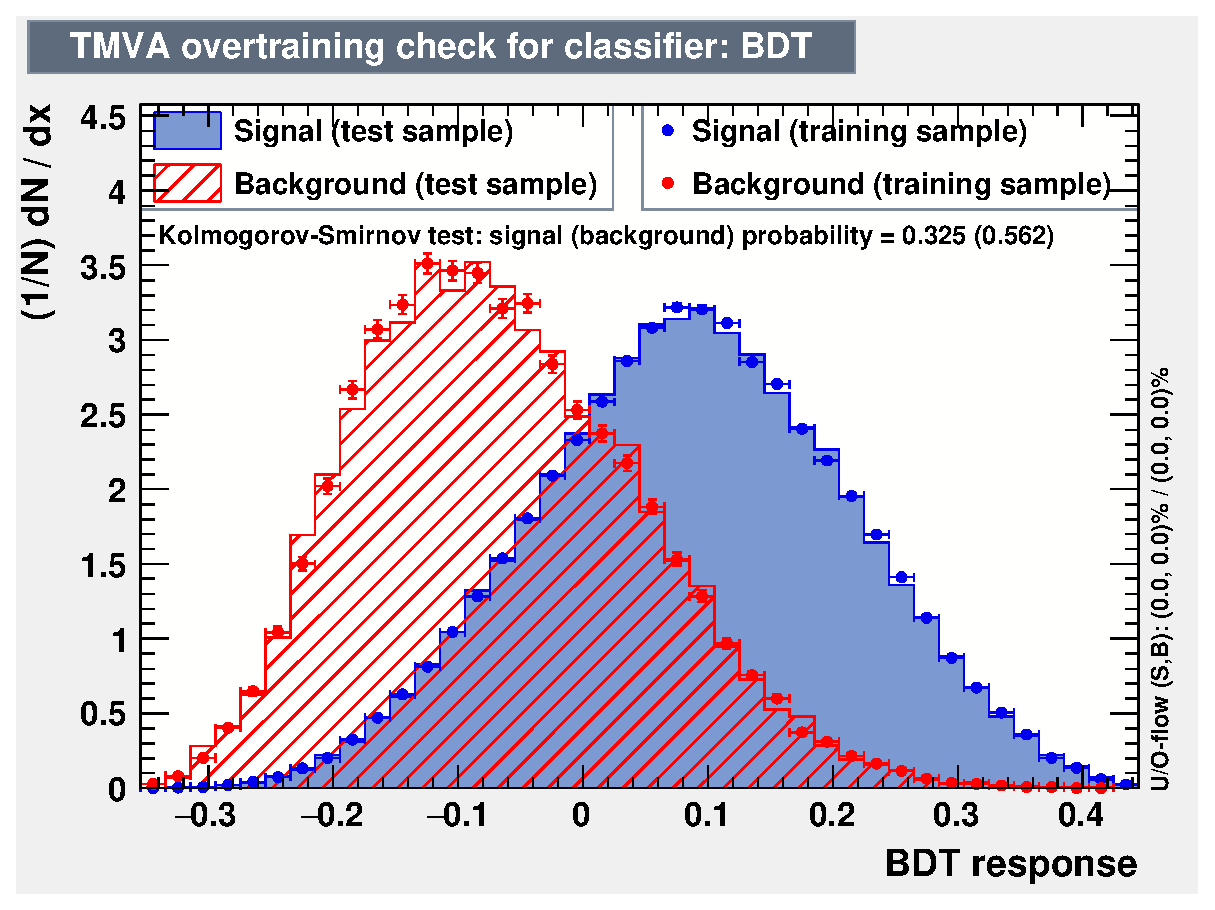
\includegraphics[width=0.45\linewidth]{figure/BDT/Perf_ggh/overtrain_BDT.eps}
  \includegraphics[width=0.45\linewidth]{figure/BDT/Perf_ggh/rejBvsS.eps}
  \caption{BDT distribution(left) and ROC curve(right) in VBF-ggF BDT training.}
  \label{fig:ROC_ggh}
\end{figure}

\begin{figure}[bp]
  \centering
  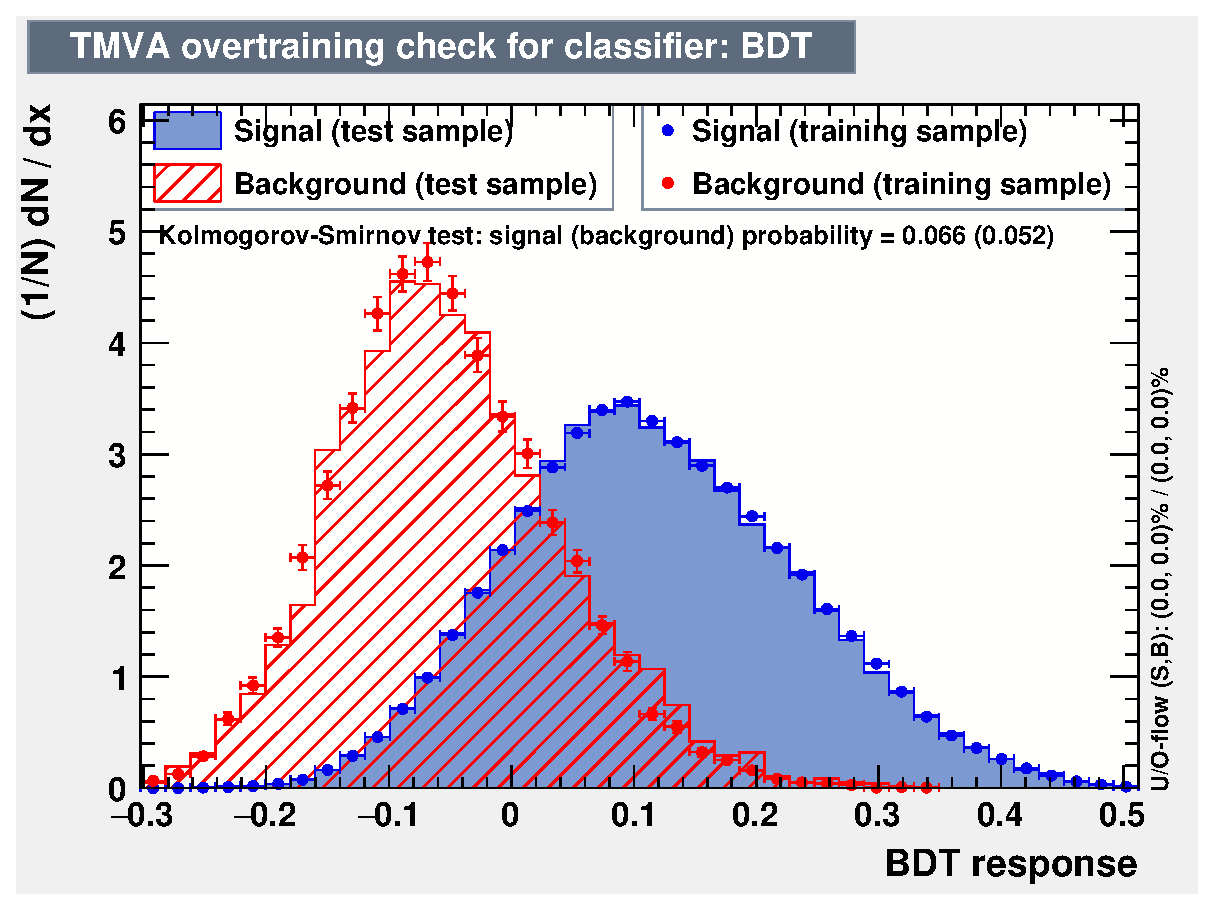
\includegraphics[width=0.45\linewidth]{figure/BDT/Perf_yy/overtrain_BDT.eps}
  \includegraphics[width=0.45\linewidth]{figure/BDT/Perf_yy/rejBvsS.eps}
  \caption{BDT distribution(left) and ROC curve(right) in VBF-$MC \gamma\gamma$ BDT training.}
  \label{fig:ROC_yy}
\end{figure}

The $BDT_{VBF/ggF}$ uses VBF purity $p= \frac{N_{VBF}}{N_{VBF}+N_{ggF}}$ as criterion. Since the maximum value of VBF purity appears at the edge of BDT range $BDT_{VBF/ggF}=1$, the working point is manually chosen to have the same VBF efficiency 34\% as in Higgs coupling categorizatio \todo{why is that?}. The VBF purity is increased from 87.7\% to 91.3\%, and gluon-fusion efficiency is decreased from 6.5\% to 4.5\%. \\

\begin{figure}[tbp]
  \centering
  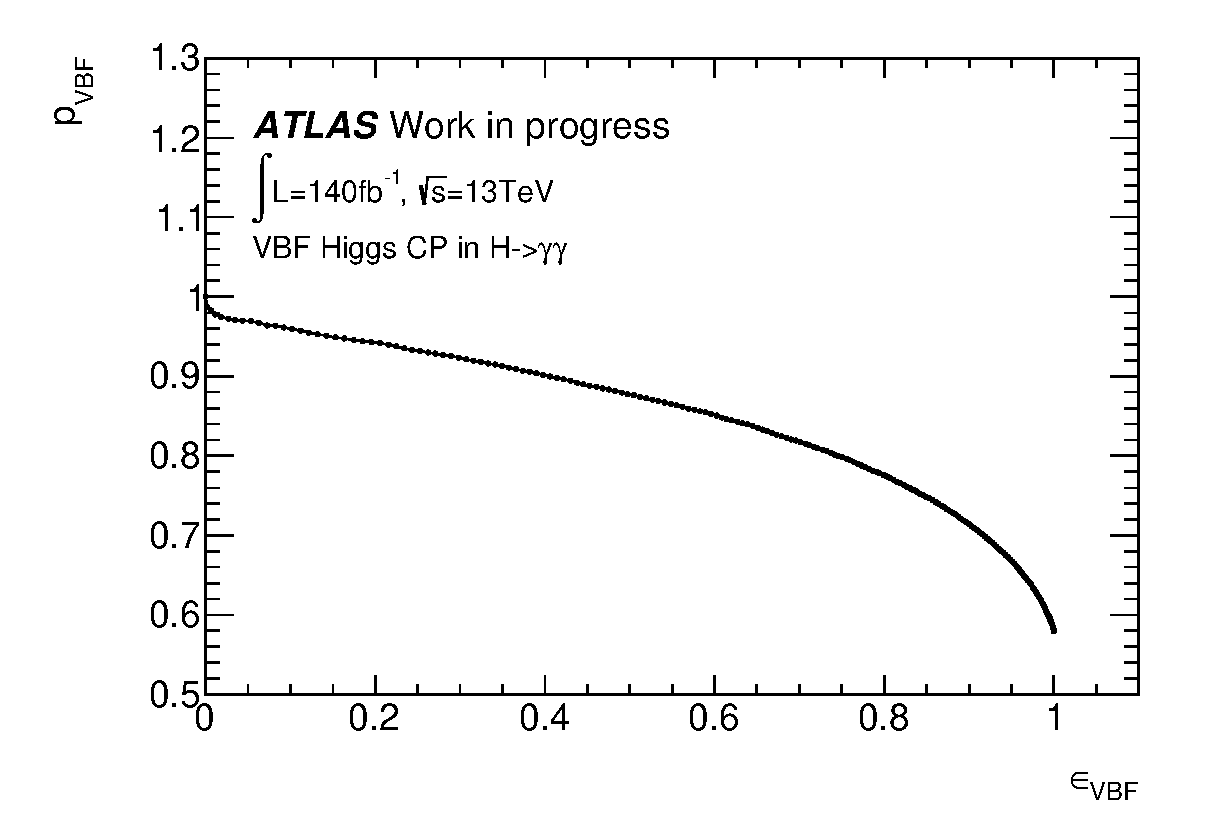
\includegraphics[width=0.45\linewidth]{figure/BDT/WP_vbfeff.eps}
  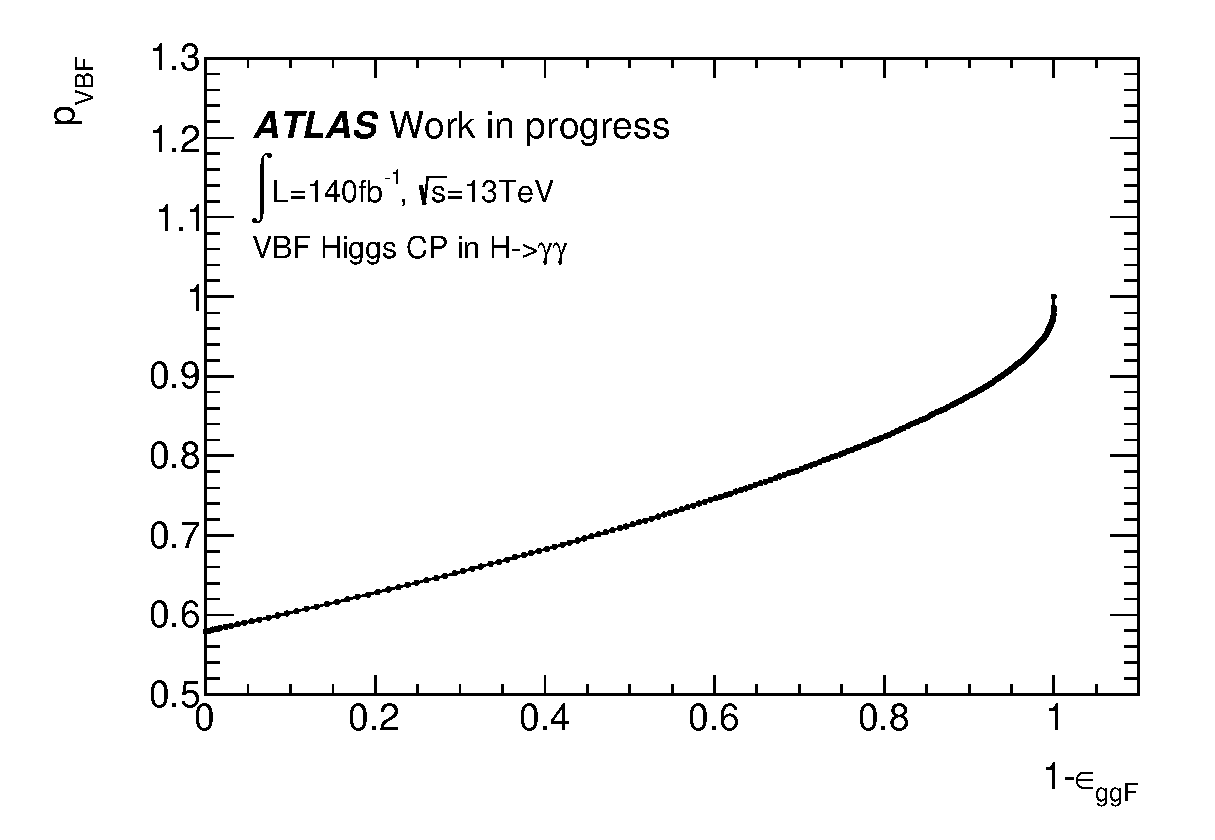
\includegraphics[width=0.45\linewidth]{figure/BDT/WP_ggfrej.eps}
  \caption{VBF purity with relationship of VBF efficiency(left) and ggF rejection(right). The working point is manually chosen with $\epsilon_{VBF}=34\%$, corresponding VBF purity and ggF rejection could be gotten.}
  \label{fig:vbfwp}
\end{figure}
\todo{explain the sudden dips/jumps in the plot}
Two regions are defined by the former criterion, naming \texttt{ggH\_tight} and \texttt{ggH\_loose} temporarily. Scanning $BDT_{VBF/\gamma\gamma}$ value in these two regions individually can provide a cut value at the global maximum VBF significance point. Figure ~\ref{fig:catedef} summary the definition of totally 4 categories, naming TT, TL, LT and LL. \\

\begin{figure}[tbp]
  \centering
  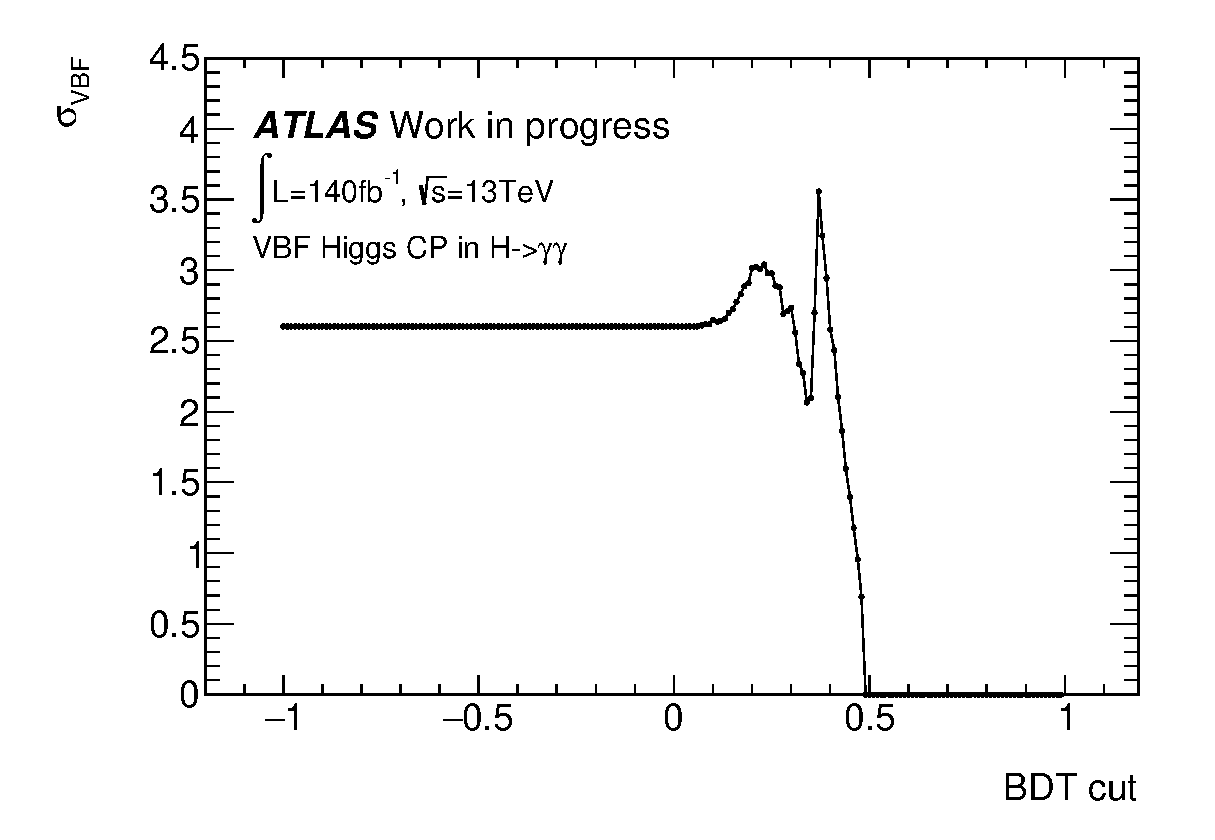
\includegraphics[width=0.45\linewidth]{figure/BDT/vbfsig_tight.eps}
  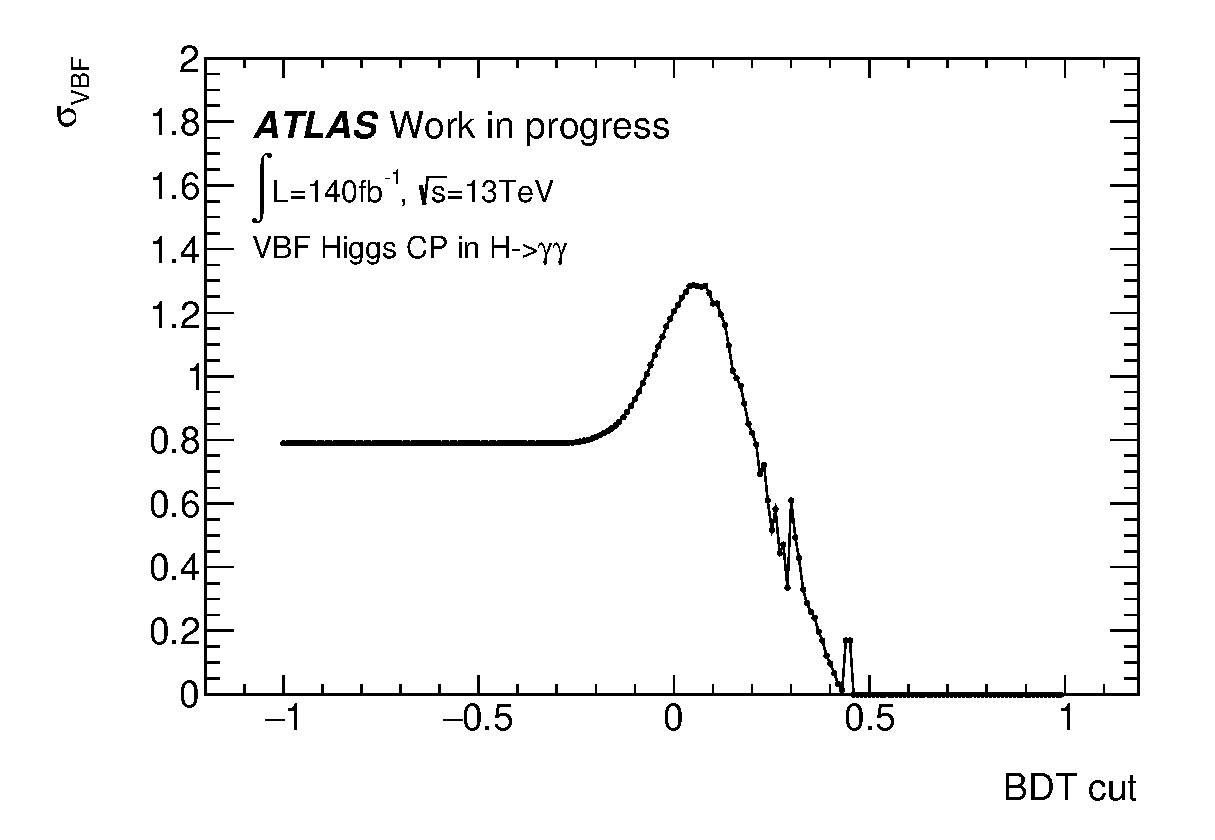
\includegraphics[width=0.45\linewidth]{figure/BDT/vbfsig_loose.eps}
  \caption{VBF significance in \texttt{ggH\_tight}(left) and \texttt{ggH\_loose}(right) regions with BDT cut value. In \texttt{ggH\_tight} the high fluctuation point has been ignored. }
  \label{fig:vbfsignificance}
\end{figure}

\begin{figure}[htbp]
  \centering
  \subfloat[]{
    \centering
    \includegraphics[width=.45\linewidth]{figure/BDT/NewCate.png}
  }
  \hfill
  \subfloat[]{
    \centering
    \begin{tabular}{ll}
      \toprule
      Category & Description \\
      \toprule
      TT       & $BDT_{VBF/ggF}>0.14, BDT_{VBF/\gamma\gamma}>0.23 $  \\
      TL       & $BDT_{VBF/ggF}>0.14, BDT_{VBF/\gamma\gamma}<0.23 $  \\
      LT       & $BDT_{VBF/ggF}<0.14, BDT_{VBF/\gamma\gamma}>0.05 $  \\
      LL       & $BDT_{VBF/ggF}<0.14, BDT_{VBF/\gamma\gamma}<0.05 $  \\
      \bottomrule
    \end{tabular}
  }
  \caption{The definition of 4 categories used in this analysis. }
  \label{fig:catedef}
\end{figure}

\begin{table}[htbp]
\centering
\begin{tabular}{|l|c|c|c|c|c|}
\hline
                  & TT    & TL     & LT      & LL       &  sum    \\ \hline
VBF               & 26.30 & 25.88  & 52.71   & 43.85    &  148.75 \\ \hline
ggF               & 1.72  & 3.22   & 24.06   & 81.77    &  110.76 \\ \hline
continuum         & 106   & 310    & 1886    & 16646    &  18949  \\ \hline
{[}120, 130{]}GeV & 21.25 & 62     & 377.25  & 3329.25  &  3789.7 \\ \hline
significance      & 5.49  & 3.20   & 2.63    & 0.75     &   \\ \hline
combined          & \multicolumn{4}{c|}{6.92}           &   \\ \hline
\end{tabular}
\label{tab:sigmaInCate}
\caption{Expectend event yields and VBF significance in 4 categories. Continuum background yield is normalized to sideband data, $[120, 130]GeV$ is estimated with background event number in full mass region times 0.2. VBF significance is calculated with background in mass window only.}
\end{table}



\subsection{Optimal observable binning}
\todo{add label for the section, use math style consistently everywhere}
The choice of optimal observable binning method can influence the sensitive of CP measurement. All events are divided into 6 positive-negative symmetry bins to ensure enough statistics and match the symmetry distribution of optimal observable \todo{use "trade-off" between purity and stats.}. With this restriction the binning can be decided by scanning only 2 parameter $p_1$ and $p_2$ with step 0.5 to have maximum global VBF significance:

%\begin{center}
%\begin{math}
$$
 Z_{\tilde{d}} = \sqrt(\Sigma_{i=0}^{6} Z_{i}^{2}) \\
 Z_{i} = Nvbf/\sqrt(Nvbf+Nggh+Nsr)
$$
%\end{math}
%\end{center}

With Nsr is the extrapolated background event number from sideband data. For different CP-mixing model the Z would be different, so in order to be model independent, an average Z value from d=-0.1 to 0.1 is chosen as the final criteria. Figure ~\ref{fig:Zvsp} shows the Z value for p1 and p2 scanning. The event number in every BDT categories and bins are shown in Table ~\ref{tab:Nevtinbins}
\todo{too short! what are the conclusions? haven't detailed how the edges where chosen}
\begin{figure}[tbp]
  \centering
  \includegraphics[width=0.45\linewidth]{figure/OObinning/binning.png}
  \includegraphics[width=0.45\linewidth]{figure/OObinning/Zscanning.png}
  \caption{The optimal observable binning is determined with 2 parameters. Global VBF significance is calculated in scanning two parameters with step of 0.5. ($p_1$, $p_2$) equal to (1, 2) and(1.5, 5,5) show very similar significance, while in order to get enough statistics in edge bins, the former one is chosen.}
  \label{fig:Zvsp}
\end{figure}

\begin{table}[htbp]
  \centering
  \subfloat[]{
  \begin{tabular}{l|ccccccc}
    VBF & {[}$-\infty$, -2{]}   & {[}-2, -1{]} & {[}-1, 0{]} & {[}0, 1{]} & {[}1, 2{]} & {[}2, $\infty${]} & sum   \\
    \toprule
    TT  & 6.29 & 3.63 & 3.22 & 3.20 & 3.63 & 6.32 & 26.30 \\ \hline
    TL  & 5.05 & 4.04 & 3.82 & 3.84 & 4.08 & 5.05 & 25.88 \\ \hline
    LT  & 8.96 & 7.72 & 9.78 & 9.65 & 7.70 & 8.90 & 52.71 \\ \hline
    LL  & 6.65 & 6.12 & 9.18 & 9.17 & 6.14 & 6.60 & 43.85 \\ 
    \bottomrule
  \end{tabular}
  }

  \subfloat[]{
  \begin{tabular}{l|ccccccc}
    ggF & {[}$-\infty$, -2{]}   & {[}-2, -1{]} & {[}-1, 0{]} & {[}0, 1{]} & {[}1, 2{]} & {[}2, $\infty${]} & sum   \\
    \toprule
    TT  & 0.28  & 0.23 & 0.33  & 0.32  & 0.26 & 0.29  & 1.72   \\ \hline
    TL  & 0.52  & 0.43 & 0.65  & 0.69  & 0.42 & 0.50  & 3.22   \\ \hline
    LT  & 3.95  & 2.76 & 5.23  & 5.31  & 2.79 & 4.02  & 24.06  \\ \hline
    LL  & 12.10 & 8.89 & 19.83 & 20.06 & 8.80 & 12.09 & 81.77  \\ 
    \bottomrule
  \end{tabular}
  }

  \subfloat[]{
  \begin{tabular}{l|ccccccc}
    Side-band data & {[}$-\infty$, -2{]}   & {[}-2, -1{]} & {[}-1, 0{]} & {[}0, 1{]} & {[}1, 2{]} & {[}2, $\infty${]} & sum   \\
    \toprule
    TT  & 18   & 13   & 13   & 12   & 13   & 16   & 85    \\ \hline
    TL  & 48   & 39   & 41   & 39   & 40   & 41   & 248   \\ \hline
    LT  & 216  & 203  & 329  & 325  & 214  & 222  & 1509  \\ \hline
    LL  & 2303 & 1539 & 2837 & 2702 & 1587 & 2349 & 13317 \\
    \bottomrule
  \end{tabular}
  }

  \label{tab:Nevtinbins}
  \caption{Expected signal event yield and sideband data number in each bins and categories. }
\end{table}


\clearpage
%%\section{Signal and background modelling}
\label{sec:model}


\subsection{Signal modelling}
\label{subsec:sigmodel}

\subsubsection{Signal yield for SM and BSM}
\label{sssec:sigyield}
\paragraph{} As discussed in Sec [ref:theory], the VBF event yields could be influenced by the additional CP-violation EFT terms. The branching ration of Higgs to diphoton $Br(H\to\gamma\gamma)$ varies from 0.227\% in SM to above 27\% in $\tilde{d}=\pm 0.01$ so that it can have a extremely strict restriction to this EFT model. Considering that the VBF process cross section can be also influenced by some other CP-conserving new physics, in the main part of this analysis ignored all restrictions from VBF event yields and only considered the OO distribution. A very preliminary result performed by both signal yield and OO shape is discussed in Appendix [ref:AppendixBr]. 

\paragraph{} The event yields for each SM process in every OO bins are displayed in Table ~\ref{tab:NevtSM}. VBF signal yields for different $\tilde{d}$ in each OO bins are in Table ~\ref{tab:NevtBSM}, total event number in all bins is scaled to SM case. These are extracted from Monte Carlo samples. 

\begin{table}[h!]
\begin{center}
\begin{tabular}{l|cccccc}
\hline
        & bin1  & bin2  & bin3  & bin4  & bin5  & bin6  \\ \hline
SM VBF  & 24.18 & 19.83 & 22.63 & 22.59 & 19.94 & 24.14 \\
ggH     & 10.70 & 12.33 & 26.16 & 26.25 & 12.25 & 10.58 \\
$\gamma\gamma$ & 1  & 1 & 1     & 1     & 1     & 1     \\ 
SB data & 1436  & 1662  & 3111  & 3048  & 1737  & 1474  \\
\hline
\end{tabular}
\caption{Event yields in 6 OO bins for each SM process and sid-band data. \textcolor{red}{h024 result. Need update to h025.}}
\label{tab:NevtSM}
\end{center}
\end{table}

\begin{table}[ht]
\begin{center}
\begin{tabular}{l|cccccc}
\hline
      & bin1  & bin2  & bin3  & bin4  & bin5  & bin6  \\ \hline
-0.1  & 47.18 & 27.37 & 26.20 & 21.50 & 16.52 & 14.77 \\
-0.09 & 44.27 & 26.43 & 25.73 & 21.50 & 16.68 & 15.11 \\
-0.08 & 41.49 & 25.53 & 25.29 & 21.52 & 16.87 & 15.57 \\
-0.07 & 38.85 & 24.67 & 24.87 & 21.57 & 17.11 & 16.18 \\
-0.06 & 36.35 & 23.86 & 24.48 & 21.64 & 17.39 & 16.91 \\
-0.05 & 33.98 & 23.08 & 24.11 & 21.73 & 17.71 & 17.78 \\
-0.04 & 31.74 & 22.35 & 23.76 & 21.86 & 18.07 & 18.78 \\
-0.03 & 29.65 & 21.66 & 23.44 & 22.00 & 18.47 & 19.92 \\
-0.02 & 27.69 & 21.01 & 23.15 & 22.17 & 18.92 & 21.19 \\
-0.01 & 25.87 & 20.40 & 22.88 & 22.37 & 19.41 & 22.60 \\
0     & 24.18 & 19.83 & 22.63 & 22.59 & 19.94 & 24.14 \\
0.01  & 22.63 & 19.30 & 22.41 & 22.84 & 20.51 & 25.82 \\
0.02  & 21.22 & 18.82 & 22.22 & 23.11 & 21.12 & 27.63 \\
0.03  & 19.94 & 18.37 & 22.05 & 23.41 & 21.78 & 29.57 \\
0.04  & 18.80 & 17.97 & 21.90 & 23.73 & 22.48 & 31.65 \\
0.05  & 17.79 & 17.60 & 21.78 & 24.08 & 23.22 & 33.86 \\
0.06  & 16.93 & 17.28 & 21.68 & 24.45 & 24.00 & 36.20 \\
0.07  & 16.19 & 17.00 & 21.61 & 24.85 & 24.82 & 38.68 \\
0.08  & 15.60 & 16.76 & 21.56 & 25.27 & 25.69 & 41.30 \\
0.09  & 15.14 & 16.56 & 21.54 & 25.72 & 26.59 & 44.05 \\
0.1   & 14.82 & 16.41 & 21.54 & 26.19 & 27.54 & 46.93 \\
\hline
\end{tabular}
\caption{BSM VBF event yields in 6 OO bins, $\tilde{d}$ varies from -0.1 to 0.1. \textcolor{red}{h024 result. Need update to h025.} }
\label{tab:NevtBSM}
\end{center}
\end{table}



\subsubsection{Signal shape}
\label{sssec:sigshape}
\paragraph{} In experiment the Higgs boson signal is described with a double-side Crystal Ball function, with the bulk modeled by a Gaussian distribution and lower tails by two independent power-low functions[ref:DSCB]. The parameters in the model are determined through fitting simulated Higgs process in each reconstructed VBF-enriched categories and OO bins. The uncertainties from signal model are considered as nuisance parameter in final systematic uncertainty estimation. 


\subsection{Background modelling}
\label{subsec:bkgmodel}
\paragraph{} The main background in this analysis are non-resonant continuum background from inclusive $\gamma\gamma$ process, and corresponding di-photon final state with one or two photons from fake jets, calling $\gamma j$ and $jj$ events. These have smoothly falling distribution in the interested $m_{\gamma\gamma}$ region and described by an empirically chosen functional form. The fraction of 3 compositions is estimated with 2x2D sideband method, while the shapes are studied as discussed in chapter [ref:bkgshape]. Then the spurious signal test is performed for determining the background model individually in each OO bins. Appendix ~\ref{appendix:2x2DSB} summaries the results of background decomposition. 

\subsubsection{Background templates derivation}
\label{ssssec:bkgtemplate}

\paragraph{} Among the three components, $\gamma\gamma$ process could be simulated with Monte Carlo, fake jet performance in $\gamma j$ and $jj$ can only be studied from data in control region due to computational limitation. Here $\gamma-j$ and $jj$ are considered together to simplify the work [\ref:HGamfiducial140]. The control region is built by inverting the tight photon identification and isolation criteria on one of the photon candidates in the final state, while all other selections are the nominal ones. This ensures enough statistics in each OO bins. $\gamma\gamma$ contamination in this control region is estimated with MC simulation and is subtracted from data, which is only a few percent. 

\paragraph{} A reweighting is performed to have further lower statistical fluctuation in this reducible background component. A smoothing function from fitting the ratio of the above control region data distribution and MC $\gamma\gamma$ distribution for events after nominal selections is used as the weight function, and this weight is applied to a high-statistics $\gamma\gamma$ MC sample. 2nd order polynomial function is selected as the fit function to the ratio. \\

\paragraph{} The total background template consists of simulated $\gamma\gamma$ and this smoothed $\gamma-j$ process. Relative fraction is calculated by 2x2D sideband method in each OO bins. The overall yield is normalized to match the side-band data in signal region. There are 3 sources of uncertainty in this template: statistics uncertainty of $\gamma\gamma$ MC, uncertainty of fraction from 2x2D, and the uncertainty of smoothing function. The first two terms are easily to obtain, the last one comes from the $m_\gamma\gamma$ distribution difference with 1st order and 2nd order polynomial as smoothing function. All these 3 terms are combined together in GPR smooth to have final background template. 

\begin{figure}[htbp]
  \centering
  \subfloat[$bin1: OO<-2$]{
  \includegraphics[width=.32\textwidth]{figure/bkg_templates/1_control_region/invID_invIso_b1.png}} 
  \subfloat[$bin2: -2<OO<-1$]{
  \includegraphics[width=.32\textwidth]{figure/bkg_templates/1_control_region/invID_invIso_b2.png}}
  \subfloat[$bin3: -1<OO<0 $]{
  \includegraphics[width=.32\textwidth]{figure/bkg_templates/1_control_region/invID_invIso_b3.png}} \\
  \subfloat[bin4: $0<OO<1$ ]{
  \includegraphics[width=.32\textwidth]{figure/bkg_templates/1_control_region/invID_invIso_b4.png}}
  \subfloat[bin5: 1<OO<2]{
  \includegraphics[width=.32\textwidth]{figure/bkg_templates/1_control_region/invID_invIso_b5.png}}
  \subfloat[bin6: 2<OO]{
  \includegraphics[width=.32\textwidth]{figure/bkg_templates/1_control_region/invID_invIso_b6.png}} \\
  \caption{Contral region sample used to estimate $\gamma j+jj$ background shape. $\gamma\gamma$ contamination has been subtracted with MC. }
  \label{fig:bkg_CR}
\end{figure}

\begin{figure}[htbp]
  \centering
  \subfloat[bin1: OO<-2]{
  \includegraphics[width=.32\textwidth]{figure/bkg_templates/2_reweight_function/invID_invIso_smooth_ratio_b1.png}} 
  \subfloat[bin2: -2<OO<-1]{
  \includegraphics[width=.32\textwidth]{figure/bkg_templates/2_reweight_function/invID_invIso_smooth_ratio_b2.png}} 
  \subfloat[bin3: -1<OO<0 ]{
  \includegraphics[width=.32\textwidth]{figure/bkg_templates/2_reweight_function/invID_invIso_smooth_ratio_b3.png}} \\
  \subfloat[bin4: 0<OO<1]{
  \includegraphics[width=.32\textwidth]{figure/bkg_templates/2_reweight_function/invID_invIso_smooth_ratio_b4.png}} 
  \subfloat[bin5: 1<OO<2]{
  \includegraphics[width=.32\textwidth]{figure/bkg_templates/2_reweight_function/invID_invIso_smooth_ratio_b5.png}} 
  \subfloat[bin6: 2<OO]{
  \includegraphics[width=.32\textwidth]{figure/bkg_templates/2_reweight_function/invID_invIso_smooth_ratio_b6.png}} \\
  \caption{Contral region data smoothed by a reweighting method.}
  \label{fig:bkg_reweight}
\end{figure}

\begin{figure}[htbp]
  \centering
  \subfloat[bin1: OO<-2]{
  \includegraphics[width=.32\textwidth]{figure/bkg_templates/3_raw_template/invID_invIso_uncertainty_b1.png}} 
  \subfloat[bin2: -2<OO<-1]{
  \includegraphics[width=.32\textwidth]{figure/bkg_templates/3_raw_template/invID_invIso_uncertainty_b2.png}} 
  \subfloat[bin3: -1<OO<0 ]{
  \includegraphics[width=.32\textwidth]{figure/bkg_templates/3_raw_template/invID_invIso_uncertainty_b3.png}} \\
  \subfloat[bin4: 0<OO<1]{
  \includegraphics[width=.32\textwidth]{figure/bkg_templates/3_raw_template/invID_invIso_uncertainty_b4.png}} 
  \subfloat[bin5: 1<OO<2]{
  \includegraphics[width=.32\textwidth]{figure/bkg_templates/3_raw_template/invID_invIso_uncertainty_b5.png}} 
  \subfloat[bin6: 2<OO]{
  \includegraphics[width=.32\textwidth]{figure/bkg_templates/3_raw_template/invID_invIso_uncertainty_b6.png}} \\
  \caption{Total background templates built with $\gamma\gamma, \gamma j+jj$ components.}
  \label{fig:bkg_total}
\end{figure}


\subsubsection{GPR smooth}
\label{sssub:GPRsmooth}

\paragraph{} In order to further remove the statistical fluctuations, the background template is smoothed with a Gaussian Process Regression (GPR) techniques. Two hyper parameters for GPR smoothing, length scale $\lambda$ and length scale slope $b_\lambda$, are optimized with a 2D space scan, which requires that smoothing out at least 33\% of narrow bump(O(bin width)) and smoothing out less than 25\% wide bump(O(signal width)) in $m_{\gamma\gamma}$ distribution. Figure ~\ref{fig:GPRdis} shows the $m_{\gamma\gamma}$ distribution before and after GPR smoothing method, comparing with the sideband data. Figure ~\ref{fig:GPRopt} shows the optimized hyper parameter spaces. 

\begin{figure}[htbp]
  \centering
  \subfloat[bin1: OO<-2]{
  \includegraphics[width=.32\textwidth]{figure/bkg_templates/4_smoothed_template/GPR_Smoothed_Plot_template_uncer_b1.png}} 
  \subfloat[bin2: -2<OO<-1]{
  \includegraphics[width=.32\textwidth]{figure/bkg_templates/4_smoothed_template/GPR_Smoothed_Plot_template_uncer_b2.png}} 
  \subfloat[bin3: -1<OO<0 ]{
  \includegraphics[width=.32\textwidth]{figure/bkg_templates/4_smoothed_template/GPR_Smoothed_Plot_template_uncer_b3.png}} \\
  \subfloat[bin4: 0<OO<1]{
  \includegraphics[width=.32\textwidth]{figure/bkg_templates/4_smoothed_template/GPR_Smoothed_Plot_template_uncer_b4.png}} 
  \subfloat[bin5: 1<OO<2]{
  \includegraphics[width=.32\textwidth]{figure/bkg_templates/4_smoothed_template/GPR_Smoothed_Plot_template_uncer_b5.png}} 
  \subfloat[bin6: 2<OO]{
  \includegraphics[width=.32\textwidth]{figure/bkg_templates/4_smoothed_template/GPR_Smoothed_Plot_template_uncer_b6.png}} \\
  \caption{Background template distribution after GPR smoothing.}
  \label{fig:GPRdis}
\end{figure}


\begin{figure}[htbp]
  \centering
  \subfloat[bin1: OO<-2]{
  \includegraphics[width=.32\textwidth]{figure/bkg_templates/GPR/GoodHyperPars_bkg_template_b1.png}} 
  \subfloat[bin2: -2<OO<-1]{
  \includegraphics[width=.32\textwidth]{figure/bkg_templates/GPR/GoodHyperPars_bkg_template_b2.png}} 
  \subfloat[bin3: -1<OO<0 ]{
  \includegraphics[width=.32\textwidth]{figure/bkg_templates/GPR/GoodHyperPars_bkg_template_b3.png}} \\
  \subfloat[bin4: 0<OO<1]{
  \includegraphics[width=.32\textwidth]{figure/bkg_templates/GPR/GoodHyperPars_bkg_template_b4.png}} 
  \subfloat[bin5: 1<OO<2]{
  \includegraphics[width=.32\textwidth]{figure/bkg_templates/GPR/GoodHyperPars_bkg_template_b5.png}} 
  \subfloat[bin6: 2<OO]{
  \includegraphics[width=.32\textwidth]{figure/bkg_templates/GPR/GoodHyperPars_bkg_template_b6.eps}} \\
  \caption{Optimized GPR hyper parameter spaces}
  \label{fig:GPRopt}
\end{figure}


\subsubsection{Spurious signal test}
\label{sssub:sstest}

\paragraph{} The final choice of background model depends on a spurious signal test. This test is done by fitting a background only shape with a signal+background function, the extracted signal yield (S) and its statistics uncertainty ($\Delta_S$) are used to measure the bias introduced by the choice of background model. The function could be accepted if it satisfy one of the following criteria: 

\begin{itemize}
\item{} $S\pm \Delta_S $ is less than 20\% of the background uncertainty
\item{} $S\pm \Delta_S $ is less than 10\% of expected signal event number. 
\end{itemize}

Tested functions include 1st, 2nd, 3rd exponential, 3,4,5 order Bernstein polynomial and first order power low function. In case not only one functions pass the criteria, the one with the fewest degree of freedom is chosen. Table ~\ref{tab:SSbin1} \~ ~\ref{tab:SSbin6} summarized the spurious signal test results and chosen background functions in 6 OO bins. 

\clearpage
\begin{landscape}

\begin{table}[]
\footnotesize
\begin{tabular}{l|ccccccccccc}
Name        & max(S/deltaS) {[}\%{]} & max(S/Sref) {[}\%{]} & max(S) & max(S) Err & nPars & chi2/ndof & Prob(chi2) {[}\%{]} & Stat Err & Stat Err {[}\%{]} & Relative Tot Err {[}\%{]} & passT0 \\ \hline
Exponential & 9.67                   & 4.84                 & 1.69   & 17.5       & 1     & 0.0327    & 100                 & 16.6     & 47.6              & 47.9                      & 1      \\
ExpPoly2    & 2.71                   & 2.56                 & 0.492  & 18.2       & 2     & 0.0134    & 100                 & 17.9     & 51.3              & 51.4                      & 1      \\
ExpPoly3    & -3.64                  & -2.15                & -0.642 & 17.6       & 3     & 0.00984   & 100                 & 18.8     & 53.9              & 53.9                      & 1      \\
Bern3       & -3.72                  & -2.49                & -0.663 & 17.8       & 3     & 0.0117    & 100                 & 19       & 54.6              & 54.6                      & 1      \\
Bern4       & -1.47                  & -1.08                & -0.276 & 18.8       & 4     & 0.0058    & 100                 & 19       & 54.6              & 54.6                      & 1      \\
Bern5       & 1.6                    & 1.35                 & 0.341  & 21.3       & 5     & 0.00178   & 100                 & 21.3     & 61.2              & 61.2                      & 1      \\
Pow         & 29.5                   & 14.1                 & 4.96   & 16.9       & 1     & 0.406     & 100                 & 16.6     & 47.6              & 49.6                      & 1      \\
\end{tabular}
\caption{Spurious signal test results for OO bin1. Exponential function is chosen.}
\label{tab:SSbin1}
\end{table}

\begin{table}[]
\footnotesize
\begin{tabular}{l|ccccccccccc}
Name        & max(S/deltaS) {[}\%{]} & max(S/Sref) {[}\%{]} &  max(S) & max(S) Err & nPars & chi2/ndof & Prob(chi2) {[}\%{]} & Stat Err & Stat Err {[}\%{]} & Relative Tot Err {[}\%{]} & passT0 \\ \hline
Exponential & 12.2                   & 6.36                 &  2.04   & 16.7       & 1     & 0.092     & 100                 & 17.6     & 54.7              & 55.1                      & 1      \\
ExpPoly2    & 6.03                   & 3.44                 &  1.11   & 18.4       & 2     & 0.0827    & 100                 & 19.1     & 59.4              & 59.5                      & 1      \\
Bern3       & -15.9                  & -10.4                &  -3.35  & 21.1       & 3     & 0.0384    & 100                 & 20.2     & 62.8              & 63.7                      & 1      \\
ExpPoly3    & -17.8                  & -12.1                &  -3.88  & 21.8       & 3     & 0.0457    & 100                 & 19.9     & 61.8              & 63                        & 1      \\
Bern4       & -15.5                  & -10.5                &  -3.35  & 21.6       & 4     & 0.0367    & 100                 & 20.2     & 62.8              & 63.6                      & 1      \\
Bern5       & -12.3                  & -8.71                &  -2.8   & 22.8       & 5     & 0.0227    & 100                 & 22.5     & 69.9              & 70.5                      & 1      \\
Pow         & 47.9                   & 24.9                 &  8.04   & 16.8       & 1     & 0.629     & 98.4                & 17.6     & 54.8              & 60.2                      & 1      \\
\end{tabular}
\caption{Spurious signal test results for OO bin2. Exponential function is chosen.}
\label{tab:SSbin2}
\end{table}

\begin{table}[]
\footnotesize
\begin{tabular}{l|ccccccccccc}
Name        & max(S/deltaS) {[}\%{]} & max(S/Sref) {[}\%{]} & max(S) & max(S) Err & nPars & chi2/ndof & Prob(chi2) {[}\%{]} & Stat Err & Stat Err {[}\%{]} & Relative Tot Err {[}\%{]} & passT0 \\ \hline
ExpPoly2    & -5.02                  & -3.26                & -1.31  & 26.2       & 2     & 0.00709   & 100                 & 25.3     & 51.8              & 51.9                      & 1      \\
ExpPoly3    & -3.08                  & -2.02                & -0.808 & 26.9       & 3     & 0.0047    & 100                 & 25.6     & 52.5              & 52.5                      & 1      \\
Bern3       & -6.48                  & -3.78                & -1.83  & 28.2       & 3     & 0.00628   & 100                 & 26.7     & 54.7              & 54.8                      & 1      \\
Bern4       & -2.85                  & -2.39                & -0.85  & 29.8       & 4     & 0.00236   & 100                 & 26.7     & 54.7              & 54.7                      & 1      \\
Bern5       & -3.66                  & -2.28                & -1.11  & 30.3       & 5     & 0.00179   & 100                 & 29.6     & 60.8              & 60.8                      & 1      \\
Pow         & 22.7                   & 10.4                 & 5.09   & 22.8       & 1     & 0.172     & 100                 & 23.2     & 47.5              & 48.6                      & 1      \\
Exponential & -35.9                  & -17.1                & -8.29  & 23.3       & 1     & 0.232     & 100                 & 23.1     & 47.4              & 50.3                      & 1     \\
\end{tabular}
\caption{Spurious signal test results for OO bin3. ExpPoly2 function is chosen.}
\label{tab:SSbin3}
\end{table}
\end{landscape}
\clearpage

\begin{landscape}
\begin{table}[]
\footnotesize
\begin{tabular}{l|ccccccccccc}
Name        & max(S/deltaS) {[}\%{]} & max(S/Sref) {[}\%{]} & max(S) & max(S) Err & nPars & chi2/ndof & Prob(chi2) {[}\%{]} & Stat Err & Stat Err {[}\%{]} & Relative Tot Err {[}\%{]} & passT0 \\ \hline
Exponential & -10.5                  & -4.71                & -2.3   & 21.9       & 1     & 0.0313    & 100                 & 23.4     & 48                & 48.2                      & 1      \\
ExpPoly2    & 12.4                   & 6.59                 & 3.22   & 25.9       & 2     & 0.0065    & 100                 & 25.6     & 52.4              & 52.8                      & 1      \\
Bern3       & 10.2                   & 5.59                 & 2.75   & 27.2       & 3     & 0.0087    & 100                 & 27       & 55.2              & 55.5                      & 1      \\
ExpPoly3    & 11                     & 6.12                 & 2.99   & 27.2       & 3     & 0.00599   & 100                 & 26.4     & 54.1              & 54.4                      & 1      \\
Bern4       & 11.2                   & 5.98                 & 3.05   & 27.6       & 4     & 0.00687   & 100                 & 27       & 55.2              & 55.6                      & 1      \\
Bern5       & 6.88                   & 4.27                 & 2.07   & 30.1       & 5     & 0.00351   & 100                 & 29.8     & 61                & 61.2                      & 1      \\
Pow         & 57.6                   & 27.9                 & 13.7   & 23.9       & 1     & 0.355     & 100                 & 23.5     & 48.1              & 55.6                      & 1      \\
\end{tabular}
\caption{Spurious signal test results for OO bin4. Exponential function is chosen.}
\label{tab:SSbin4}
\end{table}

\begin{table}[]
\footnotesize
\begin{tabular}{l|ccccccccccc}
Name        & max(S/deltaS) {[}\%{]} & max(S/Sref) {[}\%{]} &  max(S) & max(S) Err & nPars & chi2/ndof & Prob(chi2) {[}\%{]} & Stat Err & Stat Err {[}\%{]} & Relative Tot Err {[}\%{]} & passT0 \\ \hline
Exponential & 8                      & 4.81                 &  1.55   & 19.3       & 1     & 0.105     & 100                 & 18       & 56                & 56.2                      & 1      \\
ExpPoly2    & 7.04                   & 4.45                 &  1.43   & 20.3       & 2     & 0.107     & 100                 & 19.6     & 60.8              & 60.9                      & 1      \\
Bern3       & -11.8                  & -7.5                 &  -2.43  & 20.7       & 3     & 0.035     & 100                 & 20.7     & 64.3              & 64.7                      & 1      \\
ExpPoly3    & -12.5                  & -8.26                &  -2.66  & 21.4       & 3     & 0.0264    & 100                 & 20.4     & 63.3              & 63.8                      & 1      \\
Bern4       & -12.1                  & -8.12                &  -2.58  & 21.3       & 4     & 0.0316    & 100                 & 20.7     & 64.3              & 64.8                      & 1      \\
Bern5       & -6.35                  & -4.27                &  -1.48  & 23.4       & 5     & 0.00661   & 100                 & 23.1     & 71.6              & 71.8                      & 1      \\
Pow         & 39.2                   & 23.3                 &  7.56   & 19.3       & 1     & 0.586     & 99.3                & 18       & 56                & 60.7                      & 1      \\
\end{tabular}
\caption{Spurious signal test results for OO bin5. Exponential function is chosen.}
\label{tab:SSbin5}
\end{table}

\begin{table}[]
\footnotesize
\begin{tabular}{l|ccccccccccc}
Name        & max(S/deltaS) {[}\%{]} & max(S/Sref) {[}\%{]} & max(S) & max(S) Err & nPars & chi2/ndof & Prob(chi2) {[}\%{]} & Stat Err & Stat Err {[}\%{]} & Relative Tot Err {[}\%{]} & passT0 \\ \hline
Exponential & 6.56                   & 3.43                 & 1.05   & 16         & 1     & 0.0258    & 100                 & 16.6     & 47.9              & 48                        & 1      \\
ExpPoly2    & -6.2                   & -3.25                & -1.13  & 18.2       & 2     & 0.00975   & 100                 & 17.9     & 51.6              & 51.7                      & 1      \\
ExpPoly3    & -2.38                  & -1.77                & -0.487 & 20.4       & 3     & 0.00556   & 100                 & 18.8     & 54.1              & 54.1                      & 1      \\
Bern3       & -3.17                  & -2.26                & -0.629 & 19.8       & 3     & 0.00735   & 100                 & 19.1     & 54.9              & 55                        & 1      \\
Bern4       & -1.58                  & -1.42                & -0.325 & 20.6       & 4     & 0.00178   & 100                 & 19.1     & 55                & 55                        & 1      \\
Bern5       & 1.1                    & 0.967                & 0.222  & 20.3       & 5     & 0.00138   & 100                 & 21.4     & 61.6              & 61.6                      & 1      \\
Pow         & 31                     & 14.2                 & 4.97   & 16.1       & 1     & 0.341     & 100                 & 16.6     & 47.9              & 50                        & 1      \\
\end{tabular}
\caption{Spurious signal test results for OO bin6. Exponential function is chosen.}
\label{tab:SSbin6}
\end{table}

\end{landscape}




\subsection{F-test}
\label{subsec:Ftest}


\section{Signal modelling}
\label{sec:signal_model}

The shape of the signal and background \myy distributions is described with analytical functions. Like in the past analysis \cite{Hasib:2238687}, the shape of \myy invariant mass distribution for signal events in each category is modelled with a \emph{double-sided Crystal Ball} (DSCB) function. It is a composite function with 6 parameters formed by a Gaussian core, which models the peak, and two power-law tails, as detailed in \Eqn{\ref{eq:DSCB}}:
\begin{align}
	f_\text{DSCB}(\myy) = N \times
	\begin{cases}
		e^{-t^{2}/2} & \text{if } -\alpha_{low} \leq t \leq \alpha_{high} \\
		\frac{ e^{-{}^{1}_{2} \alpha_{low}^{2}} } { \left[ \frac{1}{R_{low}} \left(R_{low} - \alpha_{low} - t \right) \right]^{n_{low}} } & \text{if } t < -\alpha_{low} \\
		\frac{ e^{-{}^{1}_{2} \alpha_{high}^{2}} } { \left[ \frac{1}{R_{high}} \left(R_{high} - \alpha_{high} + t \right) \right]^{n_{high}} } & \text{if } t > \alpha_{high} \\
	\end{cases}
	\label{eq:DSCB}
\end{align}
where $N$ is a normalization factor and the six parameters are
\begin{itemize}
	\item $\mu_\text{CB}$ and $\sigma_\text{CB}$ describe the mean and the width of the Gaussian core, which are combined in $t = \left(\myy - \mu_\text{CB}\right) / \sigma_\text{CB}$;
	\item $\alpha_{low}$ and $\alpha_{high}$ are the positions of the transitions with respect to $\mu_\text{CB}$ from the Gaussian core to power-law tails, in unit of $\sigma_\text{CB}$, on the low and high mass sides respectively;
	\item $n_{low}$ and $n_{high}$ are the exponents of the low and high mass tails. With the $\alpha$'s, they define $R_{low} = \frac{n_{low}}{\alpha_{low}}$ and $R_{high}$ similarly.
\end{itemize}

In the previous analysis \cite{Hasib:2238687} \todo{which previous analysis, you meant in all HGam analysis, this is the first VBF CP analysis in HGam}, the DSCB has showed a good $\chi^2$ in the signal only fit and gives a slightly smaller\todo{smaller than what! very vague, make sure this is correct} bias on the fitted signal yield using injection tests on Asimov background and signal MC. \\ The advantage of the DSCB is to well separate the contribution coming from the core and from the tails, making easier to apply systematic variations on the scale (on $\mu_\text{CB}$) and on the resolution (to $\sigma_\text{CB}$). \\

Thanks to the very precise knowledge of the Higgs mass from Run1 from the combination of ATLAS and CMS measurements ($\mH=125.09\err{0.21}\stat\err{0.11}\syst \, \si{\GeV}$)~\cite{HIGG-2014-14} and to the relatively small error of the mass scale systematics ($<1\%$), it is possible to parametrize the shape using just one set of MC samples simulated with the Higgs mass \mH fixed at \SI{125}{\GeV}. The MC sample combines all the production modes assuming Standard Model cross sections and the three MC types (mc16a+d+e) are weighted taking into account the relative luminosity of 2015/2016, 2017 and 2018 datasets, respectively. The generalization of the fitted model to any value of \mH (in a small interval close \SI{125}{\GeV}) is done with a simple shift of the $\mu_{CB}$ parameter ($\mu_\text{CB}= m_H + \mu_\text{CB}^{\SI{125}{\GeV}} - \SI{125}{\GeV}$).\\

\textcolor{red}{Systematic from mH:  Higgs mass: 125.09 +/- 0.24 GeV as photon energy scale (PES).}
\todo{add a table with FULL variations of all PES/PER for all bins, all categories at d=0!}
The signal shapes are fitted in the fixed mass range \SIrange{105}{160}{\GeV} while leaving floating all the six parameters of the DSCB function. The signal models for each category are shown in \Fig{\ref{fig:signal_shapes}}. The same procedure is performed both for SM and BSM Monte Carlo samples, in every VBF categories, Optimal Observable bins \todo{what does that means, OO bins are determined by their best fit?!} and CP-mixing hypothesis the \myy models are determined by their best fit results from MC.

\todo{add some plots showing the up and down variations for some PES, some PER variations}

\begin{figure}[htbp]
  \includegraphics[width=.24\textwidth]{figure/sigmodel/SigFit_TTbin0.png}
  \includegraphics[width=.24\textwidth]{figure/sigmodel/SigFit_TLbin0.png}
  \includegraphics[width=.24\textwidth]{figure/sigmodel/SigFit_LTbin0.png}
  \includegraphics[width=.24\textwidth]{figure/sigmodel/SigFit_LLbin0.png}\\
  \includegraphics[width=.24\textwidth]{figure/sigmodel/SigFit_TTbin1.png}
  \includegraphics[width=.24\textwidth]{figure/sigmodel/SigFit_TLbin1.png}
  \includegraphics[width=.24\textwidth]{figure/sigmodel/SigFit_LTbin1.png}
  \includegraphics[width=.24\textwidth]{figure/sigmodel/SigFit_LLbin1.png}\\
  \includegraphics[width=.24\textwidth]{figure/sigmodel/SigFit_TTbin2.png}
  \includegraphics[width=.24\textwidth]{figure/sigmodel/SigFit_TLbin2.png}
  \includegraphics[width=.24\textwidth]{figure/sigmodel/SigFit_LTbin2.png}
  \includegraphics[width=.24\textwidth]{figure/sigmodel/SigFit_LLbin2.png}\\
  \includegraphics[width=.24\textwidth]{figure/sigmodel/SigFit_TTbin3.png}
  \includegraphics[width=.24\textwidth]{figure/sigmodel/SigFit_TLbin3.png}
  \includegraphics[width=.24\textwidth]{figure/sigmodel/SigFit_LTbin3.png}
  \includegraphics[width=.24\textwidth]{figure/sigmodel/SigFit_LLbin3.png}\\
  \includegraphics[width=.24\textwidth]{figure/sigmodel/SigFit_TTbin4.png}
  \includegraphics[width=.24\textwidth]{figure/sigmodel/SigFit_TLbin4.png}
  \includegraphics[width=.24\textwidth]{figure/sigmodel/SigFit_LTbin4.png}
  \includegraphics[width=.24\textwidth]{figure/sigmodel/SigFit_LLbin4.png}\\
  \includegraphics[width=.24\textwidth]{figure/sigmodel/SigFit_TTbin5.png}
  \includegraphics[width=.24\textwidth]{figure/sigmodel/SigFit_TLbin5.png}
  \includegraphics[width=.24\textwidth]{figure/sigmodel/SigFit_LTbin5.png}
  \includegraphics[width=.24\textwidth]{figure/sigmodel/SigFit_LLbin5.png}\\
  \caption{Fitted Doubles Sided Crystal ball shapes for all the reconstructed categories of the analysis. }
  \label{fig:signal_shapes}
\end{figure}

In the final statistical workspace:
\begin{itemize}
	\item the value of \mH is constrained to the one of \RunOne measurement, taking into account its error;
	\item all the six parameters of the DSCB are kept fix during the fit
	\item $\mu_\text{CB}$ and $\sigma_\text{CB}$ are each multiplied by a response function to take into account photon energy scale and photon energy resolution systematics, respectively (see \Sect{\ref{sssec:signal_shape_syst}} \todo{fix reference!})
\end{itemize}


\clearpage
\section{Background Modelling}
\label{sec:background_model}



\subsection{Background modeling strategy}
\label{ssec:bkg_strategy}

The strategy for the continuous background modelling follows what traditionally done in $H\to\gamma\gamma$ measurements, with the addition of some dedicated procedures to cope with specific issues related to insufficient MC statistics or very low-statistics categories. This section only contains a simplified description, more details could be found in HGam coupling analysis ~\ref{ANA-HIGG-2020-16-INT1}. 

The steps comprising the background modelling strategy can be summarised as follows:
\begin{itemize}

  \item The composition of the continuous background in term of \yy, \yjet and \jetjet components is estimated with data driven technique for each category entering the measurement, as detailed in \Sect{\ref{ssec:bkg_composition}}.
  \item The background fractions are used to build \myy background templates for each category entering the measurement, where the \yy component is obtained from MC, while the \yjet and \jetjet components are measured from data driven control regions and used to reweight the \yy MC, as detailed in \Sect{\ref{ssec:bkg_templates}}.

  \item In order to improve the background modeling and reduce the impact of limited MC statistics, a smoothing procedure is being developed to be eventually applied to the background template, provided that the improvements on the results outweight the possible associated systematic uncertainties. 

  \item The Spurious Signal approach is used in the smoothed \yy templates to select a functional form to describe each template, as well as the associated bias that will enter the measurement as a systematic uncertainties, as detailed in \Sect{\ref{ssec:spurious_signal}}. The Spurious Signal criteria are defined in order to cope with the limited MC statistics that in some case leads to non-physical large bias measurements.

  \item In very low-statistic categories, defined as those categories with \textcolor{red}{less than 10 events per bin in the \myy sidebands}, the smoothing procedure tends to introduce large non-physical structures in the templates, and it is therefore not suited to be used for them. For this reason, for this categories we initially select the statistically-justified function performing a Wald-test on the data sidebands using a family of function based on a exponential of increasing complexity. We accept the simplest function justifies by the Wald-test, and perform the Spurious Signal measurement with this function tolerating a bias that could be larger than the criteria used for the high-statistic categories, but would have a small impact on the overall sensitivity. This procedure is described in \Sect{\ref{sssec:bkg_functions}}. 

\end{itemize}


\subsection{Background compositions}
\label{ssec:bkg_composition}

The dominant background entering the invariant mass spectrum comes from SM continuum diphoton production. A large number of photons are produced inside jets due to de decays of neutral mesons to photon pairs. Thus, photon-jet and di-jet events in which the jets are mis-identified as photons represent a non-negligible source of background. Photon-pairs can be also faked from Drell-Yan events in which both electrons are misidentified as photons. However, this background only contributes with a small fraction ($<1\%$).

The number of \yy, \yjet and \jetjet events entering each category after the final selection is estimated by means of a double two-dimensional sideband ABCD method~\cite{ATL-COM-PHYS-2012-592}. This data-driven method extrapolates the fraction of fake photons within the signal region from the composition of the side-band control regions, built by inverting photon identification and isolation requirements. The fractions are calculated individually in each categories and OO bins for the background template building. Table ~\ref{tab:yyfraction} lists the \yy fraction in all categories. More details are shown in Appendix ~\ref{appendix:2x2DSB}. 

\begin{table}[htbp]
  \centering
  \begin{tabular}{c|cccc}
  \toprule
           &  TT  &  TL  &  LT  &  LL  \\ 
  \toprule
  OO bin1  & $0.76 \pm 0.16$ & $0.90 \pm 0.10$ & $0.93 \pm 0.03$ & $0.86 \pm 0.05$ \\ \hline
  OO bin2  & $0.89 \pm 0.10$ & $0.81 \pm 0.10$ & $0.81 \pm 0.06$ & $0.87 \pm 0.07$ \\ \hline
  OO bin3  & $0.79 \pm 0.15$ & $0.75 \pm 0.12$ & $0.88 \pm 0.03$ & $0.83 \pm 0.06$ \\ \hline
  OO bin4  & $0.92 \pm 0.08$ & $0.81 \pm 0.09$ & $0.84 \pm 0.05$ & $0.90 \pm 0.05$ \\ \hline
  OO bin5  & $0.78 \pm 0.14$ & $0.81 \pm 0.10$ & $0.86 \pm 0.05$ & $0.88 \pm 0.07$ \\ \hline
  OO bin6  & $0.88 \pm 0.10$ & $0.87 \pm 0.09$ & $0.88 \pm 0.05$ & $0.83 \pm 0.04$ \\
  \bottomrule
  \end{tabular}
  \caption{\yy fraction calculated with double two-dimensional sideband ABCD method. \yjet and \jetjet components are merged together in following analysis, so the fraction is $1-f_{\yy}$. }
  \label{tab:yyfraction}
\end{table}

\begin{figure}[tbp]
  \centering
  \includegraphics[width=0.45\linewidth]{figure/bkgtmpls/TT/yyfrac_TT.png}
  \includegraphics[width=0.45\linewidth]{figure/bkgtmpls/TL/yyfrac_TL.png} \\
  \includegraphics[width=0.45\linewidth]{figure/bkgtmpls/LT/yyfrac_LT.png}
  \includegraphics[width=0.45\linewidth]{figure/bkgtmpls/LL/yyfrac_LL.png} 
  \caption{\yy, \yjet, \jetjet fraction in TT(upper left), TL(upper right), LT(bottom left), LL(bottom right) categories, as a function of OO. }
  \label{fig:yyfraction}
\end{figure}



\clearpage
\subsection{Background templates}
\label{ssec:bkg_templates}

Considering the low \jetjet fraction and similar performance of \yjet and \jetjet, those two components are merged together as \yjet+\jetjet for the background estimation. The shape is determined with a data control region, in TT, TL and LT categories it is defined as at least one of the two selected photons fail the tight identification and loose isolation requirement due to insufficient MC statistics, and in LL category it is defined as inverting the identification and isolation of exactly one of two photon candidates.
Contamination from \yy has been tested to be ignorable as shown in Figure ~\ref{fig:yjCR}, and a \textcolor{red}{linear} reweighting is derived to match the \yy and control region shapes. The bin width for ratio function smoothing varies from 5GeV, 2GeV, 1GeV and 0.5GeV respectively in TT, TL, LT, LL categories to match the MC statistics for an un-biased result. Uncertainty of this reweighted template contains two part: from the choice of smoothing function and from \yy fraction, while the latter is dominant. 
These derived shapes are combined with the measured relative event fractions to obtain the total background shape. The \yy fraction is measured as mentioned in ~\ref{ssec:bkg_composition} \\

The obtained templates show a good agreement when comparing them with events in data passing the nominal selection (with tight photon identification and isolation cuts, TI) in the sidebands, as shown in \Fig{\ref{fig:BkgData-MC}}.\\

\clearpage
\begin{figure}[htbp]
  \centering
  \subfloat[TT category OO bin1]{ \includegraphics[width= 0.30\textwidth]{figure/bkgtmpls/TT/CR/b1.png} }
  \subfloat[TT category OO bin2]{ \includegraphics[width= 0.30\textwidth]{figure/bkgtmpls/TT/CR/b2.png} }
  \subfloat[TT category OO bin3]{ \includegraphics[width= 0.30\textwidth]{figure/bkgtmpls/TT/CR/b3.png} } \\
  \subfloat[TT category OO bin4]{ \includegraphics[width= 0.30\textwidth]{figure/bkgtmpls/TT/CR/b4.png} }
  \subfloat[TT category OO bin5]{ \includegraphics[width= 0.30\textwidth]{figure/bkgtmpls/TT/CR/b5.png} }
  \subfloat[TT category OO bin6]{ \includegraphics[width= 0.30\textwidth]{figure/bkgtmpls/TT/CR/b6.png} } \\
  \subfloat[TL category OO bin1]{ \includegraphics[width= 0.30\textwidth]{figure/bkgtmpls/TL/CR/b1.png} }
  \subfloat[TL category OO bin2]{ \includegraphics[width= 0.30\textwidth]{figure/bkgtmpls/TL/CR/b2.png} }
  \subfloat[TL category OO bin3]{ \includegraphics[width= 0.30\textwidth]{figure/bkgtmpls/TL/CR/b3.png} } \\
  \subfloat[TL category OO bin4]{ \includegraphics[width= 0.30\textwidth]{figure/bkgtmpls/TL/CR/b4.png} }
  \subfloat[TL category OO bin5]{ \includegraphics[width= 0.30\textwidth]{figure/bkgtmpls/TL/CR/b5.png} }
  \subfloat[TL category OO bin6]{ \includegraphics[width= 0.30\textwidth]{figure/bkgtmpls/TL/CR/b6.png} } \\
\end{figure}
\clearpage
\begin{figure}[htbp]
\centering
  \subfloat[LT category OO bin1]{ \includegraphics[width= 0.30\textwidth]{figure/bkgtmpls/LT/CR/b1.png} }
  \subfloat[LT category OO bin2]{ \includegraphics[width= 0.30\textwidth]{figure/bkgtmpls/LT/CR/b2.png} }
  \subfloat[LT category OO bin3]{ \includegraphics[width= 0.30\textwidth]{figure/bkgtmpls/LT/CR/b3.png} } \\
  \subfloat[LT category OO bin4]{ \includegraphics[width= 0.30\textwidth]{figure/bkgtmpls/LT/CR/b4.png} }
  \subfloat[LT category OO bin5]{ \includegraphics[width= 0.30\textwidth]{figure/bkgtmpls/LT/CR/b5.png} }
  \subfloat[LT category OO bin6]{ \includegraphics[width= 0.30\textwidth]{figure/bkgtmpls/LT/CR/b6.png} } \\
  \subfloat[LL category OO bin1]{ \includegraphics[width= 0.30\textwidth]{figure/bkgtmpls/LL/CR/b1.png} }
  \subfloat[LL category OO bin2]{ \includegraphics[width= 0.30\textwidth]{figure/bkgtmpls/LL/CR/b2.png} }
  \subfloat[LL category OO bin3]{ \includegraphics[width= 0.30\textwidth]{figure/bkgtmpls/LL/CR/b3.png} } \\
  \subfloat[LL category OO bin4]{ \includegraphics[width= 0.30\textwidth]{figure/bkgtmpls/LL/CR/b4.png} }
  \subfloat[LL category OO bin5]{ \includegraphics[width= 0.30\textwidth]{figure/bkgtmpls/LL/CR/b5.png} }
  \subfloat[LL category OO bin6]{ \includegraphics[width= 0.30\textwidth]{figure/bkgtmpls/LL/CR/b6.png} } \\
  \caption{Control region data in all categories and OO bins.}
  \label{fig:yjCR}
\end{figure}
\clearpage

\begin{figure}[htbp]
  \centering
  \subfloat[TT category OO bin1]{ \includegraphics[width= 0.30\textwidth]{figure/bkgtmpls/TT/reweight/b1.png} }
  \subfloat[TT category OO bin2]{ \includegraphics[width= 0.30\textwidth]{figure/bkgtmpls/TT/reweight/b2.png} }
  \subfloat[TT category OO bin3]{ \includegraphics[width= 0.30\textwidth]{figure/bkgtmpls/TT/reweight/b3.png} } \\
  \subfloat[TT category OO bin4]{ \includegraphics[width= 0.30\textwidth]{figure/bkgtmpls/TT/reweight/b4.png} }
  \subfloat[TT category OO bin5]{ \includegraphics[width= 0.30\textwidth]{figure/bkgtmpls/TT/reweight/b5.png} }
  \subfloat[TT category OO bin6]{ \includegraphics[width= 0.30\textwidth]{figure/bkgtmpls/TT/reweight/b6.png} } \\
  \subfloat[TL category OO bin1]{ \includegraphics[width= 0.30\textwidth]{figure/bkgtmpls/TL/reweight/b1.png} }
  \subfloat[TL category OO bin2]{ \includegraphics[width= 0.30\textwidth]{figure/bkgtmpls/TL/reweight/b2.png} }
  \subfloat[TL category OO bin3]{ \includegraphics[width= 0.30\textwidth]{figure/bkgtmpls/TL/reweight/b3.png} } \\
  \subfloat[TL category OO bin4]{ \includegraphics[width= 0.30\textwidth]{figure/bkgtmpls/TL/reweight/b4.png} }
  \subfloat[TL category OO bin5]{ \includegraphics[width= 0.30\textwidth]{figure/bkgtmpls/TL/reweight/b5.png} }
  \subfloat[TL category OO bin6]{ \includegraphics[width= 0.30\textwidth]{figure/bkgtmpls/TL/reweight/b6.png} } \\
\end{figure}
\clearpage
\begin{figure}[htbp]
\centering
  \subfloat[LT category OO bin1]{ \includegraphics[width= 0.30\textwidth]{figure/bkgtmpls/LT/reweight/b1.png} }
  \subfloat[LT category OO bin2]{ \includegraphics[width= 0.30\textwidth]{figure/bkgtmpls/LT/reweight/b2.png} }
  \subfloat[LT category OO bin3]{ \includegraphics[width= 0.30\textwidth]{figure/bkgtmpls/LT/reweight/b3.png} } \\
  \subfloat[LT category OO bin4]{ \includegraphics[width= 0.30\textwidth]{figure/bkgtmpls/LT/reweight/b4.png} }
  \subfloat[LT category OO bin5]{ \includegraphics[width= 0.30\textwidth]{figure/bkgtmpls/LT/reweight/b5.png} }
  \subfloat[LT category OO bin6]{ \includegraphics[width= 0.30\textwidth]{figure/bkgtmpls/LT/reweight/b6.png} } \\
  \subfloat[LL category OO bin1]{ \includegraphics[width= 0.30\textwidth]{figure/bkgtmpls/LL/reweight/b1.png} }
  \subfloat[LL category OO bin2]{ \includegraphics[width= 0.30\textwidth]{figure/bkgtmpls/LL/reweight/b2.png} }
  \subfloat[LL category OO bin3]{ \includegraphics[width= 0.30\textwidth]{figure/bkgtmpls/LL/reweight/b3.png} } \\
  \subfloat[LL category OO bin4]{ \includegraphics[width= 0.30\textwidth]{figure/bkgtmpls/LL/reweight/b4.png} }
  \subfloat[LL category OO bin5]{ \includegraphics[width= 0.30\textwidth]{figure/bkgtmpls/LL/reweight/b5.png} }
  \subfloat[LL category OO bin6]{ \includegraphics[width= 0.30\textwidth]{figure/bkgtmpls/LL/reweight/b6.png} } \\
  \caption{Reweight \yy MC with a linear function to match the \yjet+\jetjet shape in each bins and categories.}
  \label{fig:yyReweight}
\end{figure}
\clearpage

\begin{figure}[htbp]
  \centering
  \subfloat[TT category OO bin1]{ \includegraphics[width= 0.30\textwidth]{figure/bkgtmpls/TT/raw_tmpl/b1.png} }
  \subfloat[TT category OO bin2]{ \includegraphics[width= 0.30\textwidth]{figure/bkgtmpls/TT/raw_tmpl/b2.png} }
  \subfloat[TT category OO bin3]{ \includegraphics[width= 0.30\textwidth]{figure/bkgtmpls/TT/raw_tmpl/b3.png} } \\
  \subfloat[TT category OO bin4]{ \includegraphics[width= 0.30\textwidth]{figure/bkgtmpls/TT/raw_tmpl/b4.png} }
  \subfloat[TT category OO bin5]{ \includegraphics[width= 0.30\textwidth]{figure/bkgtmpls/TT/raw_tmpl/b5.png} }
  \subfloat[TT category OO bin6]{ \includegraphics[width= 0.30\textwidth]{figure/bkgtmpls/TT/raw_tmpl/b6.png} } \\
  \subfloat[TL category OO bin1]{ \includegraphics[width= 0.30\textwidth]{figure/bkgtmpls/TL/raw_tmpl/b1.png} }
  \subfloat[TL category OO bin2]{ \includegraphics[width= 0.30\textwidth]{figure/bkgtmpls/TL/raw_tmpl/b2.png} }
  \subfloat[TL category OO bin3]{ \includegraphics[width= 0.30\textwidth]{figure/bkgtmpls/TL/raw_tmpl/b3.png} } \\
  \subfloat[TL category OO bin4]{ \includegraphics[width= 0.30\textwidth]{figure/bkgtmpls/TL/raw_tmpl/b4.png} }
  \subfloat[TL category OO bin5]{ \includegraphics[width= 0.30\textwidth]{figure/bkgtmpls/TL/raw_tmpl/b5.png} }
  \subfloat[TL category OO bin6]{ \includegraphics[width= 0.30\textwidth]{figure/bkgtmpls/TL/raw_tmpl/b6.png} } \\
\end{figure}
\clearpage
\begin{figure}[htbp]
\centering
  \subfloat[LT category OO bin1]{ \includegraphics[width= 0.30\textwidth]{figure/bkgtmpls/LT/raw_tmpl/b1.png} }
  \subfloat[LT category OO bin2]{ \includegraphics[width= 0.30\textwidth]{figure/bkgtmpls/LT/raw_tmpl/b2.png} }
  \subfloat[LT category OO bin3]{ \includegraphics[width= 0.30\textwidth]{figure/bkgtmpls/LT/raw_tmpl/b3.png} } \\
  \subfloat[LT category OO bin4]{ \includegraphics[width= 0.30\textwidth]{figure/bkgtmpls/LT/raw_tmpl/b4.png} }
  \subfloat[LT category OO bin5]{ \includegraphics[width= 0.30\textwidth]{figure/bkgtmpls/LT/raw_tmpl/b5.png} }
  \subfloat[LT category OO bin6]{ \includegraphics[width= 0.30\textwidth]{figure/bkgtmpls/LT/raw_tmpl/b6.png} } \\
  \subfloat[LL category OO bin1]{ \includegraphics[width= 0.30\textwidth]{figure/bkgtmpls/LL/raw_tmpl/b1.png} }
  \subfloat[LL category OO bin2]{ \includegraphics[width= 0.30\textwidth]{figure/bkgtmpls/LL/raw_tmpl/b2.png} }
  \subfloat[LL category OO bin3]{ \includegraphics[width= 0.30\textwidth]{figure/bkgtmpls/LL/raw_tmpl/b3.png} } \\
  \subfloat[LL category OO bin4]{ \includegraphics[width= 0.30\textwidth]{figure/bkgtmpls/LL/raw_tmpl/b4.png} }
  \subfloat[LL category OO bin5]{ \includegraphics[width= 0.30\textwidth]{figure/bkgtmpls/LL/raw_tmpl/b5.png} }
  \subfloat[LL category OO bin6]{ \includegraphics[width= 0.30\textwidth]{figure/bkgtmpls/LL/raw_tmpl/b6.png} } \\
  \caption{Final background templates.}
  \label{fig:BkgData-MC}
\end{figure}
\clearpage


\subsubsection{Background smoothing}
\label{ssec:bkg_smoothing}
\textcolor{red}{Need Simplification} \\

Because of the limited statistics of the simulation samples used in the calculation, the value
of the spurious signal systematic uncertainty is subject to significant statistical fluctuations within
many of the analysis categories~\cite{Hyneman:2712576}. Statistical fluctuations in the background-only sample may cause
signal-like bumps, which are then fit as signal by the spurious signal procedure. These statistical fluctuations do
not capture the shape mismodeling from the analytic function, and they often drastically inflate the
value of the systematic.

Although simply producing additional simulation samples would alleviate the issue of statistical
fluctuations fitted as spurious signal, producing more simulated events is computationally
expensive. Additionally, producing events which fall into specific phase spaces is often highly inefficient. 
Therefore, an alternative solution using the available simulation samples is preferred. 

A Gaussian Process (GP) is defined as a set of random processes, where all finite subsets of these
processes have a multivariate normal distribution~\cite{ebden2015gaussian}. 
Given a finite dataset – such as the bin contents of a smooth histogram – with corresponding
mean and covariance matrices, a Gaussian Process may be defined. The “correct” mean and the
covariance, however, are not necessarily well defined, as they encode specific assumptions about
the underlying dataset. In practice, the two quantities are fit to a finite dataset using a minimization
algorithm. In the case of a one-dimensional histogram with a finite number of bins, the mean can
be interpreted as a “rough” description of the underlying shape. The diagonal elements of the
covariance matrix represent the error of each bin while the off-diagonal elements specify
how “similar” the bin content of two different bins should be.

The covariance matrix can be simplified through the introduction of a kernel, which analytically
determines the level of correlation between two distinct points (i.e., the length scales in X at which points are expected to influence one another in Y). Two useful kernels are the Radial Basis Function (RBF) kernel and the Gibbs kernel~\cite{3569,Gibbs}. 

The RBF kernel has one hyperparameter, the constant length scale $l$, and it is defined as

\begin{equation}
K_\text{RBF}(x,x') = exp\left(\frac{-(x-x')^2}{2l^2}\right)
\end{equation}

The RBF kernel is useful for mostly-flat functions. However, for smoothly-falling functions, it is likely that nearby points will be more correlated in some regions than in others, so a constant length scale is a suboptimal model. The Gibbs kernel allows the length scale $l(x)$ to vary linearly as a function of $x$, and thus has two hyperparameters: the initial length scale and the length scale slope. The Gibbs kernel function is: 

\begin{equation}
K_\text{Gibbs}(x, x') = \frac{\sqrt{2l(x)l(x')}}{l(x)^2 + l(x')^2 } \cdot exp\left( \frac{-(x-x')^2}{l(x)^2 + l(x')^2} \right)
\end{equation}


The background templates used in the spurious signal test for the analysis categories are all smooth,
roughly exponentially falling distributions with statistical fluctuations. Fitting a background template
using Gaussian Process Regression (using the Gibbs kernel with the errors as determined by the initial templates) 
offers a consistent method of estimating the underlying smooth shape of the template, without the problematic fluctuations. 
Notably, the GP smoothing technique makes no assumption on the underlying distribution other than that it is smooth and falling, hence the choice of functional form from the spurious signal test will not be biased.

The hyperparameters (initial length scale and length scale slope) are allowed to vary over a range specified by the user; the optimal hyperparameters within this range are determined by the Gaussian Process fitting procedure.

A GP is fit to the original (noisy) background template in each category. The GP mean in the fits is defined as an exponential function,
the parameters of which are obtained by a fit to the original background template. The exponential
shape has been observed to be a sufficiently close guess for the categories used by the analysis.
However, in cases where the input template has very few statistics (less than about ten events per
bin on average), the resulting GP fit may be nearly identical to the mean exponential shape. This
issue occurs when the statistical uncertainties of the original template are so large that the template
is fully compatible with the preliminary exponential shape. Although the exponential shape
is technically an adequate descriptor of the template shape, the choice of the exponential mean
does bias the functional choice of the spurious signal test in this case. Therefore, a check has been
added to re-perform the GP fit using a flat mean in cases where the resulting GP shape and the
mean exponential shape disagree with a $\chi^2/DoF < 0.1$.

The resulting smoothed shape obtained from the GP fit is then saved as a new histogram. This
smoothed histogram is passed as the background template to the spurious signal test, which then
determines the background functional form and spurious signal systematic uncertainty as described
in \Sect{\ref{ssec:spurious_signal}}.

Note that based on previous study, the GPR method can only remain effectively unbiased for smoothly-falling templates containing more than an average of 20 Monte Carlo events/ bin ~\cite{ATLAS-CONF-2020-026}. 
The TT and TL categories in this analysis even do not have sufficient statistics for GPR. Only LT and LL categories used this method, and the treatment of TT and TL is discussed in Section ~\ref{sssec:bkg_functions}. 

Examples of the smoothed templates are presented in \Fig{\ref{fig:exampleGPR}} for a sample category with a high
level of statistics and for a category with a very low level of statistics.
The original templates are shown as well, for comparison. The data sidebands are also shown for
validation, although the GP smoothing technique does not take into account the data sidebands.

\begin{figure}[htbp]
  \centering
  \subfloat[LT category OO bin1]{ \includegraphics[width= 0.30\textwidth]{figure/bkgtmpls/LT/smooth_tmpl/b1.png} }
  \subfloat[LT category OO bin2]{ \includegraphics[width= 0.30\textwidth]{figure/bkgtmpls/LT/smooth_tmpl/b2.png} }
  \subfloat[LT category OO bin3]{ \includegraphics[width= 0.30\textwidth]{figure/bkgtmpls/LT/smooth_tmpl/b3.png} } \\
  \subfloat[LT category OO bin4]{ \includegraphics[width= 0.30\textwidth]{figure/bkgtmpls/LT/smooth_tmpl/b4.png} }
  \subfloat[LT category OO bin5]{ \includegraphics[width= 0.30\textwidth]{figure/bkgtmpls/LT/smooth_tmpl/b5.png} }
  \subfloat[LT category OO bin6]{ \includegraphics[width= 0.30\textwidth]{figure/bkgtmpls/LT/smooth_tmpl/b6.png} } \\
  \subfloat[LL category OO bin1]{ \includegraphics[width= 0.30\textwidth]{figure/bkgtmpls/LL/smooth_tmpl/b1.png} }
  \subfloat[LL category OO bin2]{ \includegraphics[width= 0.30\textwidth]{figure/bkgtmpls/LL/smooth_tmpl/b2.png} }
  \subfloat[LL category OO bin3]{ \includegraphics[width= 0.30\textwidth]{figure/bkgtmpls/LL/smooth_tmpl/b3.png} } \\
  \subfloat[LL category OO bin4]{ \includegraphics[width= 0.30\textwidth]{figure/bkgtmpls/LL/smooth_tmpl/b4.png} }
  \subfloat[LL category OO bin5]{ \includegraphics[width= 0.30\textwidth]{figure/bkgtmpls/LL/smooth_tmpl/b5.png} }
  \subfloat[LL category OO bin6]{ \includegraphics[width= 0.30\textwidth]{figure/bkgtmpls/LL/smooth_tmpl/b6.png} } \\
  \caption{LT and LL category background templates after GPR smooth.}
  \label{fig:exampleGPR}
\end{figure}


%The smoothed background templates used in this analysis and the spurious signal values extracted from them can be found in the \App{\ref{sec:GPR_templates}}.


%Extensive validation tests were performed with the GP smoothing technique in order to ensure that the smoothing itself does not introduce a substantial bias. These tests primarily use “toy” templates – randomly-generated background templates constructed from either simulated diphoton events or from the probability distribution function of a known analytic function. We find that GPR remains effectively unbiased for smoothly-falling templates containing more than an average of 20 Monte Carlo events/ bin. These procedures to validate the GPR smoothing are reported in \App{\ref{sec:GPR_validation}}.





\subsection{Spurious signal test}
\label{ssec:spurious_signal}

The background \myy shape, for each analysis category, is described using an analytic function whose parameters and normalization are fitted to data. The choices for the analytic function that has been considered are:
\begin{itemize}
\item Exponential Function: $f(\myy) = e^{c\cdot \myy}$
\item Exponential Function of $2^{nd}$ Order Polynomial: $f(\myy) = e^{c_1\cdot m^2_{\gamma\gamma}+c_2\cdot \myy}$
\item Exponential Function of $3^{nd}$ Order Polynomial: $f(\myy) = e^{c_1\cdot m^3_{\gamma\gamma}+c_2\cdot m^2_{\gamma\gamma}+c_3\cdot \myy}$
\item Bernstein polynomial of order $N$: $B_{N}(\myy) = \sum_{i=0}^N c_i\cdot b_{i,N}$ with $b_{i,N} = \begin{pmatrix}N\\i\end{pmatrix}\myy^i (1-\myy)^{N-i}$, N=3, 4, 5
\item First-Order Power Law Function: $f(\myy) = \myy^c$
\end{itemize}
The method to select the functional form in each category is based on the spurious signal. The spurious signal test is described in more detail in \cite{Hasib:2238687}.

To perform the spurious signal test, the full analytic signal plus background model is fitted to a background-only template for each category separately. The fit is performed in the nominal diphoton mass range of $105 \leq \myy \leq \SI{160}{\GeV}$. The number of fitted signal events as a function of the Higgs mass is computed in intervals of \SI{1}{\GeV} within the diphoton mass range of $120 \leq \myy \leq \SI{130}{GeV}$. Negative fluctuations are taken into account. The number of spurious signal events $N_{sp}$ is then defined as the maximum of the absolute value of the fitted number of signal events within the signal diphoton mass sub-range. The statistical error is always taken into account.

The choice of analytic function is done such that the function satisfies at least one of the following criteria:
\begin{itemize}
\item $N_{sp}$ < 10\% $N_{s,exp}$, where $N_{s,exp}$ is the expected number of signal events within the SM in the category ($\mu_{sp} = N_{sp} / N_{s,exp}$)
\item $N_{sp}$ < 20\% $\sigma_{bkg}$, where $\sigma_{bkg}$ is the statistical uncertainty on the fitted number of signal events, when fitting the signal+background model to a background only Asimov dataset ($Z_{sp} = N_{sp} / \sigma_{bkg}$).
\end{itemize}

If multiple functions pass the test, then the one with the least number of parameters is chosen.

%The study including all the categories (also non-ttH) will be performed in the future in accordance with the method described in the previous iteration of the analysis. Due to the higher statistics, new functions (with more parameters) might be needed for the high statistics event categories, as for example the ggH categories. For the ttH only analysis, this does not need to be done.
%These should pass at least the 
%Due to the limitation of MC statistic amount, 
    A relaxed spurious signal criteria, that are made to accommodate $2\sigma$ local statistical fluctuations in the MC template, in case the MC statistics is small compared to the expected signal. This is done by defining a new variable:
\begin{align}
    \zeta_{sp} = 
   \begin{cases}
N_{sp} + 2\Delta_{MC},~~~~ N_{sp} + 2\Delta_{MC}<0\\
N_{sp} - 2\Delta_{MC},~~~~ N_{sp} - 2\Delta_{MC}>0\\
0, ~~~~~~~~~~~~~~~~~~~~~~~\text{otherwise}\\
\end{cases}
 \label{eq:relSpuriousSignalMetric}
\end{align}
where $\Delta_{MC}$ is a local statistical fluctuation of the MC background template. This is illustrated in \Fig{\ref{fig:relaxed_ss_cartoon}}. This newly defined variable should then pass the criteria as $N_{sp}$ before. 

For categories with at least 100 data events in the sideband regions defined as $105 < m_{\gamma\gamma} < 120$ GeV or $130 < m_{\gamma\gamma} < 160$ GeV, the background functions are selected to result in a $|S_{\text{spur}}|$ that is smaller than either 10\% of the total expected Higgs boson signal event ($S_{\text{exp}}$) or 20\% of the statistical uncertainty of the fitted signal yield ($\sigma_{\text{exp}}$). The fit of the analytic function to the background template is required to yield a $\chi^2$ probability of at least $1\%$~\footnote{The $\chi^2$ is computed with a background template uniformly binned over $105<m_{\gamma\gamma}<160$ GeV. The number of bins is 22, and the degrees of freedom used in the computation is 21 - $N_{\text{pars}}$, the number of free function parameters.}.

If multiple functions pass the requirements, the one with the smallest number of degrees of freedom is chosen. If no function passes, the spurious signal requirement is relaxed to  
 $\zeta_{sp}$ < 10\% $N_{s,exp}$ or $\zeta_{sp}$ < 20\% $\sigma_{bkg}$.
For 28 out of the 88 categories, these relaxed conditions were used. 
It's to be emphasized that even the relaxed condition is used, the background uncertainty is still $N_{sp}$ from the nominal approach of spurious signal study.





\subsubsection{Treatment of low-statistic cetegories}
\label{sssec:bkg_functions}

The determination of analytical functions is part of the result of spurious signal study, however, for low stastics categories with a background template suffering of very large statistical flucttuation we introduce a preliminary step. The straight use of the spurious signal procedure on these templates, in fact, would potentially lead to select a function with large number of degrees of freedom to accomodate these statistical fluctuation, and these function can prove to be dangerous when used on data. For this reason, for categories with less then 100 events in the \myy\ sidebads, we restrict the selection of the modeling function to exponential of first, second and third order, collectively described by:
\begin{equation}
  f_i{x} = e^{\sum_{i=0}^2 a_i x^i}
\end{equation}
where $x = \myy$. 

We accept as modeling function the $f_i$ function with the lowest number of degrees of freedom for which the addition of more degrees of freedom does not lead to a significant improvement in the quality of the fit of the \myy\ sidebands. 
To this purpose, we checked the likelihood ratio between the fits to the side-band data with two different background models:
\begin{equation}
\lambda_{(1,2)} = -2ln(L_{1}/L_{2})
\end{equation}
Where $L_{1}$ and $L_{2}$ are the likelihood values of the two fits.

The distributions of these test statistics are computed with \myy\
 side-band data, fitting it with two models and calculating the value of the test statistics.  
 Once the distributions of the test-statistics
are computed, we can reject the simpler (less parameters) background
model by checking the P-value $P(\lambda >= \lambda_{\mathrm{data}})$ with the $\lambda$ measured in data ($\lambda_{\mathrm{data}}$).
This procedure to reject simpler background function is called Wald test.

Figure ~\ref{fig:Wtest} shows plots of the Wald-test on the low-statistic categories. All of the categories selected exponential function as the final decison.
Where the lowest P-value among all categories are around 3$\%$, corresponding to a significance of 2.2 $\sigma$ standard deviations.  
The background uncertainty for these categories will be the spurious signal from exponential function.

As a cross-check, a F-test is also performed in Appendix ~\ref{append:ss}, and we draw the same conclusion that all of the categories can select exponential function.
The reason we use Wald test to decide the background function is the fits on side-band data are un-bin fit (so that it's consistent with the final result), 
    there might be bias if we calculate the $\chi^2$ values in an artifical bin-size for the F-test. In this case the Wald test based on likelihood ratio is more reliable.

\begin{figure}[htbp]
  \centering
  \subfloat[TT category OO bin1]{ \includegraphics[width= 0.30\textwidth]{figure/bkgtmpls/TT/wald/b1.png} }
  \subfloat[TT category OO bin2]{ \includegraphics[width= 0.30\textwidth]{figure/bkgtmpls/TT/wald/b2.png} }
  \subfloat[TT category OO bin3]{ \includegraphics[width= 0.30\textwidth]{figure/bkgtmpls/TT/wald/b3.png} } \\
  \subfloat[TT category OO bin4]{ \includegraphics[width= 0.30\textwidth]{figure/bkgtmpls/TT/wald/b4.png} }
  \subfloat[TT category OO bin5]{ \includegraphics[width= 0.30\textwidth]{figure/bkgtmpls/TT/wald/b5.png} }
  \subfloat[TT category OO bin6]{ \includegraphics[width= 0.30\textwidth]{figure/bkgtmpls/TT/wald/b6.png} } \\
  \subfloat[TL category OO bin1]{ \includegraphics[width= 0.30\textwidth]{figure/bkgtmpls/TL/wald/b1.png} }
  \subfloat[TL category OO bin2]{ \includegraphics[width= 0.30\textwidth]{figure/bkgtmpls/TL/wald/b2.png} }
  \subfloat[TL category OO bin3]{ \includegraphics[width= 0.30\textwidth]{figure/bkgtmpls/TL/wald/b3.png} } \\
  \subfloat[TL category OO bin4]{ \includegraphics[width= 0.30\textwidth]{figure/bkgtmpls/TL/wald/b4.png} }
  \subfloat[TL category OO bin5]{ \includegraphics[width= 0.30\textwidth]{figure/bkgtmpls/TL/wald/b5.png} }
  \subfloat[TL category OO bin6]{ \includegraphics[width= 0.30\textwidth]{figure/bkgtmpls/TL/wald/b6.png} } \\
  \caption{Wald test in TT and TL categories. In all OO bins the first order exponential function shows the lower p value and is selected.}
  \label{fig:Wtest}
\end{figure}




\subsection{Background modelling results}
\label{ssec:bck_results}

The determined analytical functions modeling the baground in each category entering the measureument are found in Table~\ref{tab:spurious_sig} , as well as the corresponsing Spurious Signal bias.
The background only fit on the background templates based on MC samples is shown in Figure ~\ref{fig:bkgonly}


\begin{table}[htbp]
\centering
\small
\begin{tabular}{l|l|l|l|l|l|l|l|l}
\hline
           & \multicolumn{2}{c|}{TT} & \multicolumn{2}{c|}{TL} & \multicolumn{2}{c|}{LT} & \multicolumn{2}{c|}{LL} \\ \hline
           & Selected func. & maxS   & Selected func. & maxS   & Selected func. & maxS   & Selected func. & maxS   \\ \hline \hline
bin0       & Exp            & -0.29  & Exp            & -0.468 & Exp            & 0.87   & Exp            & 0.885  \\ \hline
bin1       & Exp            & 0.582  & Exp            & -0.882 & Exp            & -0.534 & Exp            & 1.54   \\ \hline
bin2       & Exp            & 0.235  & Exp            & -0.355 & Pow            & 0.437  & ExpPoly2       & -1.64  \\ \hline
bin3       & Exp            & 0.409  & Exp            & -0.304 & Pow            & 0.642  & Exp            & -0.718 \\ \hline
bin4       & Exp            & -0.404 & Exp            & 0.779  & Exp            & 0.775  & Exp            & -1.19  \\ \hline
bin5       & Exp            & 0.293  & Exp            & 0.408  & Exp            & 0.627  & Exp            & 0.52   \\ \hline
\end{tabular}
\caption{The final background modelling decision and the size of spurious signal uncertainties.}
\label{tab:spurious_sig}
\end{table}


\begin{figure}[htbp]
  \centering
  \subfloat[TT category OO bin1]{ \includegraphics[width= 0.30\textwidth]{figure/bkgfit/TT/b1.pdf} }
  \subfloat[TT category OO bin2]{ \includegraphics[width= 0.30\textwidth]{figure/bkgfit/TT/b2.pdf} }
  \subfloat[TT category OO bin3]{ \includegraphics[width= 0.30\textwidth]{figure/bkgfit/TT/b3.pdf} } \\
  \subfloat[TT category OO bin4]{ \includegraphics[width= 0.30\textwidth]{figure/bkgfit/TT/b4.pdf} }
  \subfloat[TT category OO bin5]{ \includegraphics[width= 0.30\textwidth]{figure/bkgfit/TT/b5.pdf} }
  \subfloat[TT category OO bin6]{ \includegraphics[width= 0.30\textwidth]{figure/bkgfit/TT/b6.pdf} } \\
  \subfloat[TL category OO bin1]{ \includegraphics[width= 0.30\textwidth]{figure/bkgfit/TL/b1.pdf} }
  \subfloat[TL category OO bin2]{ \includegraphics[width= 0.30\textwidth]{figure/bkgfit/TL/b2.pdf} }
  \subfloat[TL category OO bin3]{ \includegraphics[width= 0.30\textwidth]{figure/bkgfit/TL/b3.pdf} } \\
  \subfloat[TL category OO bin4]{ \includegraphics[width= 0.30\textwidth]{figure/bkgfit/TL/b4.pdf} }
  \subfloat[TL category OO bin5]{ \includegraphics[width= 0.30\textwidth]{figure/bkgfit/TL/b5.pdf} }
  \subfloat[TL category OO bin6]{ \includegraphics[width= 0.30\textwidth]{figure/bkgfit/TL/b6.pdf} } \\
\end{figure}
\clearpage
\begin{figure}[htbp]
\centering
  \subfloat[LT category OO bin1]{ \includegraphics[width= 0.30\textwidth]{figure/bkgfit/LT/b1.pdf} }
  \subfloat[LT category OO bin2]{ \includegraphics[width= 0.30\textwidth]{figure/bkgfit/LT/b2.pdf} }
  \subfloat[LT category OO bin3]{ \includegraphics[width= 0.30\textwidth]{figure/bkgfit/LT/b3.pdf} } \\
  \subfloat[LT category OO bin4]{ \includegraphics[width= 0.30\textwidth]{figure/bkgfit/LT/b4.pdf} }
  \subfloat[LT category OO bin5]{ \includegraphics[width= 0.30\textwidth]{figure/bkgfit/LT/b5.pdf} }
  \subfloat[LT category OO bin6]{ \includegraphics[width= 0.30\textwidth]{figure/bkgfit/LT/b6.pdf} } \\
  \subfloat[LL category OO bin1]{ \includegraphics[width= 0.30\textwidth]{figure/bkgfit/LL/b1.pdf} }
  \subfloat[LL category OO bin2]{ \includegraphics[width= 0.30\textwidth]{figure/bkgfit/LL/b2.pdf} }
  \subfloat[LL category OO bin3]{ \includegraphics[width= 0.30\textwidth]{figure/bkgfit/LL/b3.pdf} } \\
  \subfloat[LL category OO bin4]{ \includegraphics[width= 0.30\textwidth]{figure/bkgfit/LL/b4.pdf} }
  \subfloat[LL category OO bin5]{ \includegraphics[width= 0.30\textwidth]{figure/bkgfit/LL/b5.pdf} }
  \subfloat[LL category OO bin6]{ \includegraphics[width= 0.30\textwidth]{figure/bkgfit/LL/b6.pdf} } \\
  \caption{Background only fit on the background templates based on MC samples. }
  \label{fig:bkgonly}
\end{figure}



\clearpage
\section{Systematic uncertainties}
\label{sec:syst}


\subsection{Theory uncertainties}
\label{ssec:theoryuncert}
The estimation of the CP BSM parameters from the OO shape requires the precise knowledge of the SM contributions and related uncertainties. This includes both SM gluon-gluon fusion (background) and SM VBF (signal).
 Therefore, the different theoretical uncertainties affecting the SM predictions are included in the fitting likelihood. This includes uncertainties from PDF, QCD order and $\alpha_s$.

For the gluon-fusion production mode, nine uncertainty sources are used to model the QCD theory
uncertainties, following the recommendation of the LHC Higgs cross section working group~\cite{LHCXS_4}. These sources are:
\begin{itemize}
\item two sources correspond to yield uncertainties related to the total cross section. Their magnitude is taken from the
STWZ-BLPTW predictions~\cite{ggF_qcd_unc_1,ggF_qcd_unc_2,LHCXS_4} and their impact on the different bins is evaluated using
NNLOPS.
\item two sources correspond to migration uncertainties related to splitting the phase space by jet multiplicity. Their magnitude and impact are derived similarly to the yield uncertainties
\item two uncertainty sources are related to the $p_\mathrm{T}^H$ shape and are estimated from scale
variations in NNLOPS, including variations of the HNNLO input scales and the renormalization
and factorization scales in Powheg.
\item two uncertainty sources related to the enhancement of uncertainties for events with typical VBF topology (due to explicit or implicit third-jet vetos), and are estimated by scale variations in MCFM~\cite{MCFM}, and the corresponding uncertainties are estimated using the same procedure use for yield and migration uncertainties.
\item one uncertainty source is related to the treatment of $m_t$ and is most important at large $p_\mathrm{T}^H$.
\end{itemize}

Following the recommendations of PDF4LHC~\cite{pdf4lhc}, the PDF uncertainties are evaluated using the 30 eigenvectors set and treating each of them as an uncorrelated source. One additional nuisance parameter accounts for the uncertainties in $\alpha_{s}$.

For the $VBF+VH$ production modes, QCD uncertainties are estimated as an envelope of the scale variations available in Powheg~\cite{Nason:2009ai,VBFVH_theoryUnc}. Uncertainties from the choice of the PDF set and $\alpha_\mathrm{s}$ are evaluated similar to the gluon-fusion case.
A summary of the magnitude of these uncertainties in the different categories and OO bins is shown in the Figure ~\ref{fig:theoryUnc_ggF} ~\ref{fig:theoryUnc_VBF}.

\begin{figure}[htbp]
\centering
  \subfloat[TT ]{ \includegraphics[width= 0.23\textwidth]{figure/TheorySyst/ggF_theoryUnc_TT_d_0.pdf} }
  \subfloat[TL ]{ \includegraphics[width= 0.23\textwidth]{figure/TheorySyst/ggF_theoryUnc_TL_d_0.pdf} }
  \subfloat[LT ]{ \includegraphics[width= 0.23\textwidth]{figure/TheorySyst/ggF_theoryUnc_LT_d_0.pdf} } 
  \subfloat[LL ]{ \includegraphics[width= 0.23\textwidth]{figure/TheorySyst/ggF_theoryUnc_LL_d_0.pdf} } 
  \caption{Theory uncertainty in different OO bins for ggF process}
  \label{fig:theoryUnc_ggF}
\end{figure}

\begin{figure}[htbp]
\centering
  \subfloat[TT ]{ \includegraphics[width= 0.23\textwidth]{figure/TheorySyst/VBF_theoryUnc_TT_d_0.pdf} }
  \subfloat[TL ]{ \includegraphics[width= 0.23\textwidth]{figure/TheorySyst/VBF_theoryUnc_TL_d_0.pdf} }
  \subfloat[LT ]{ \includegraphics[width= 0.23\textwidth]{figure/TheorySyst/VBF_theoryUnc_LT_d_0.pdf} }
  \subfloat[LL ]{ \includegraphics[width= 0.23\textwidth]{figure/TheorySyst/VBF_theoryUnc_LL_d_0.pdf} }
  \caption{Theory uncertainty in different OO bins for VBF process}
  \label{fig:theoryUnc_VBF}
\end{figure}




\subsection{Uncertainties from signal and background modeling}
\label{ssec:modeluncert}

\paragraph{} The Higgs peak described by double-side crystal ball function can be influence by several experimental effects. 
Photon energy scale uncertainties shift the position of signal peak by between $\pm0.2\%$ and $\pm0.4\%$, while the photon resolution uncertainties change the width of signal peak by between $\pm 6\%$ and $\pm 15\%$, following Ref ~\cite{ref:phscaleres}. 
Uncertainty due to knowledge of Higgs boson mass of 0.24GeV ~\cite{ref:mHerror} would also affect the signal peak position. 
These sources are considered independently into systematic uncertainties. 
\# \textcolor{red}{NUMBER NEED CHECK}

\paragraph{} The uncertainty due to the background choice is taken to be the spurious signal yield discussed in \Sect{\ref{ssec:spurious_signal}}, and assumed to be uncorrelated in each bins. 


\subsection{Experimental systematic uncertainties affecting the expected signal yields}
\label{ssec:expuncert}

\paragraph{} With data taken during 2015-2018, the uncertainty from integrate luminosity is 2.0\% \textcolor{red}{(NEED VARIFICATION)}. Other sources of experimental uncertainty affecting the expected signal yields include: the efficiency of diphoton trigger, the photon identification and isolation efficiencies, the photon energy scale and resolution, the modelling of pile-up in the simulation, the jet energy scale and resolution, the efficiency of the jet vertex tagger. Among them the dominant one is Pile-up reweight \texttt{ATLAS\_PRW\_DATASF} which contributes 4\%. \\

The considered systematic uncertainty terms are shown in Figure ~\ref{fig:syst_ranking}. 

\begin{figure}[h]
  \centering
  \includegraphics[width=.9\textwidth]{figure/ranking_allcats.pdf}
  \caption{Ranking plot for all systematic uncertainty terms. }
  \label{fig:syst_ranking}
\end{figure}



\clearpage
\section{Fitting strategy}
\label{sec:fit}
\todo{Add what is fixed and what is float in the likelihood, details that this is shape analysis, detail the constraint function (Gaussian, or log-normal and for which NPs), add asimov plots for signal+Bkg fits, add the NP-ranking plots, add detailed NLL curves and table with numbers using stat-only, stat+sys, breakdown of jet and photon sys for different categories}
\paragraph{} The estimation of CP-mixing parameter $\tilde{d}$ uses a maximum-likelihood fit performed on $m_{\gamma\gamma}$ distribution simultaneously in all 6 OO bins. The likelihood function could be constructed as:

\begin{center}
\begin{math}
\mathcal{L}(\boldsymbol{x} |\mu_{vbf},N_{bkg},p_{bkg},\boldsymbol{\theta}) = \prod_{i}^{bin}Pois(n_{i}|\nu_{i}(\mu_{vbf},\boldsymbol{\theta}))\prod_{j=1}^{N}f_{i}(m_{\gamma\gamma}^{j};\boldsymbol{\theta})\prod_{k}G(\theta_{k})
\end{math}
\end{center}

\begin{center}
	\begin{math}
	f_{i}(m_{\gamma\gamma})\propto(\mu_{vbf} \times N_{vbf}^{i} + N_{ggF}^{i})\times f_{sig}(m_{\gamma\gamma};\boldsymbol{p_{CB}^{i}})+N_{bkg}^{i}\times f_{bkg}(m_{\gamma\gamma};\boldsymbol{p_{bkg}^{i}})
	\end{math}
\end{center}

\begin{center}
\begin{math}
\nu_{i}=
\end{math}
\end{center}

where,
\begin{itemize}
	\item $\boldsymbol x$ represents dataset
	\item VBF signal strength, $\mu_{vbf}$, is the POI and shared among all the bins in the fit
	\item the following NPs are float in the fit: continuum background yields ($N_{bkg}$) , continuum background shape parameters ($\boldsymbol{p_{bkg}}$) and other systematic NPs ($\boldsymbol{\theta}$)
	\item signal yields ($N_{vbf}$, $N_{ggF}$) and shape parameters ($\boldsymbol{p_{CB}}$) of signal function are fixed to MC prediction
	\item $f_{i}(m_{\gamma\gamma})$ is the diphoton invariant mass distribution model for each bins
	\item double sided crystal ball function is used for $f_{sig}$
	\item $f_{bkg}$ are either selected by spurious signal test or by wald test as described in \Sect{\ref{sec:background_model}}
	\item $G(\boldsymbol \theta)$ are constraint functions for systematic uncertainties as in Table~\ref{tab:constraint_func}
\end{itemize}

\begin{table}[]
	\centering
\begin{tabular}{ccc}
	\hline
	\toprule
	\multicolumn{2}{c}{systematic} & constraint funciton \\ \hline
	\toprule
	\multirow{2}{*}{exp.}  & jet    & asymmetric                \\ \cline{2-3} 
	& photon & asymmetric                \\ \hline
	\multirow{3}{*}{theo.} & PDF    & log-nornmal                \\ \cline{2-3} 
	& QCD    & log-normal                \\ \cline{2-3} 
	& shower & Gaussian                \\ \bottomrule
\end{tabular}
\caption{constraint functions for systematics}
\label{tab:constraint_func}
\end{table}

The parameter of interest (POI) of this analysis, $\tilde{d}$, is embedded in $m_{\gamma\gamma}$ model, so there is no analytic relation between likelihood value and POI. A set of signal templates corresponding to different value of CP-mixing parameter $\tilde{d}$ is created by reweighting the SM VBF $H\to\gamma\gamma$ to build the CP-mixing models, and then a template fit could be performed with data and model with different $\tilde{d}$ value (background model kept\todo{kept} consistent) to evaluate the likelihood function. For the fit in each $\tilde{d}$ model, VBF signal strength, continuum background yield and parameters describing the background model are float, which means the effect of background mis-modelling is considered and any constrain from possible model-dependent cross section information is not exploited. Other nuisance parameters are fixed to their best-fit values $\hat{\boldsymbol \theta}$. 


\paragraph{} A negative log-likelihood (NLL) curve can be constructed by calculating the NLL value for each $\tilde{d}$ hypothesis. Best-estimated $\tilde{d}$ as well as its central confidence interval at 68\% (95\%) confidence level (CL) can be determined with the minimum value of NLL, $NLL_{min}$ and the points at which $\Delta NLL = NLL-NLL_{min} = 0.5(1.96)$. An Asimov dataset is used to get expected sensitivity from this method and is shown in Figure ~\ref{fig:NLLcurve}. 


\paragraph{} Since the Optimal Observable is the main sensitive variable for CP test in this analysis, another 2D model for OO and $m_\gamma\gamma$ was considered to construct the likelihood function. In some preliminary study this 2D model did not show significant improvement with baseline method, and had some difficulty in modelling, it was obsoleted in this analysis. Appendix ~\ref{appendix:2Dmodel} includes some results based on this. 



\clearpage
\section{Results}
\label{sec:result}

For a CP-even Higgs boson, the mean value of Optimal Observable is expected to be 0 for both signal and background process. So a direct and totally model independent measurement of Higgs CP could be obtained from this with data. Table ~\ref{tab:meanOO} shows the observed mean Optimal Observable value in data and the statistical uncertainties. 

\begin{table}[]
\centering
\begin{tabular}{ll}
\hline
         & \textless{}OO\textgreater{} \\ \hline \hline
TT       &   $  0.014 \pm 4.004 $      \\ \hline
TL       &   $ -0.004 \pm 3.895 $      \\ \hline
LT       &   $ -0.013 \pm 3.752 $      \\ \hline
LL       &   $ -0.006 \pm 3.879 $      \\ \hline \hline
combined &                             \\ \hline
\end{tabular}
\caption{Mean values of Optimal Observable and statistical only uncertainty in 4 categories and their combination. }
\label{tab:meanOO}
\end{table}


A more precise measurement of CP-mixing parameter $\tilde{d}$ is performed with a maximum likelihood fit described in Section ~\ref{sec:fit}. The parameter of interest $\tilde{d}$ is scanned with step of 0.01 and other nuisance parameters are adjusted within their allowed constraints. Table ~\ref{tab:dtilde_mu_obs} summarized the best fit signal strength and $\tilde{d}$ with statistical and systematic uncertainty. Expected results from MC is shown in Table ~\ref{tab:dtilde_mu_exp}. \\

The expected and observed $\Delta NLL$ curve is shown in figure ~\ref{fig:NLLcurve} as a function of $~\tilde{d}$. In the expected result the signal strength is set to 1, and $\tilde{d}$ is set to 0, corresponding to the best estimate of sensitivity of the analysis based on SM prediction. The contribution from 4 categories are shown with statistical only $\Delta NLL$ curve in Figure ~\ref{fig:NLLcurve_4cate}. 

\begin{table}[]
\centering
\small
\begin{tabular}{lcccc}
\toprule
         & $\mu \pm unc.(stat.)$ &  $\tilde{d}\pm unc.(stat.)(68\% interval)$   & 95\% interval of $\tilde{d}$(stat.) & 95\% interval of $\tilde{d}$(stat.+syst.)  \\
\toprule
TT       &  $1.00\pm0.27 (0.25)$  &  $0.00^{+0.039(0.039)}_{-0.039(0.038)}$      &  $ [-0.092, 0.096] $                &  $ [-0.094, 0.099] $                       \\ \hline
TL       &  $1.00\pm0.36 (0.34)$  &  $0.00^{+0.062(0.061)}_{-0.062(0.061)}$      &  $ [-0.272, 0.254] $                &  $ [-0.295, 0.273] $                       \\ \hline
LT       &  $1.00\pm0.38 (0.35)$  &  $0.00^{+0.062(0.061)}_{-0.061(0.060)}$      &  $ [-0.303, 0.315] $                &  $ [-0.329, 0.337] $                       \\ \hline
LL       &  $1.00\pm1.12 (1.12)$  &  $0.00^{+1.407(1.197)}_{-1.293(1.148)}$      &  $ [-4.924, 5.071] $                &  $ [-5.551, 6.023] $                       \\
\bottomrule
combined &  $1.00\pm0.20 (0.17)$  &  $0.00^{+0.027(0.027)}_{-0.027(0.026)}$      &  $ [-0.057, 0.059] $                &  $ [-0.059, 0.060] $                       \\ 
\bottomrule
\end{tabular}
\caption{Expected results for signal strength and $\tilde{d}$. }
\label{tab:dtilde_mu_exp}
\end{table}

\begin{figure}[h]
  \centering
  \includegraphics[width=.7\textwidth]{figure/NLLcurve.png}
  \caption{Expected $\Delta NLL$ curve for combined result. }
  \label{fig:NLLcurve}
\end{figure}

\begin{figure}[h]
  \centering
  \includegraphics[width=.7\textwidth]{figure/NLLcurve_4cate.png}
  \caption{Statistical only $\Delta NLL$ curve for 4 categories. }
  \label{fig:NLLcurve_4cate}
\end{figure}




\clearpage
\section{Conclusion}
\label{sec:conclusion}

The CP invariance of Higgs boson coupling to vector bosons has been tested in VBF \Hyy process with $140 fb^{-1}$ 13TeV proton-proton collision data collected by ATLAS detector in its full Run2 period. The measurement is performed in differential Optimal Observable region within SMEFT model, the BSM Higgs coupling contributing to CP are represented with $c_{HW}$, xxx, xxx. \\

\#Results 


\clearpage

%-------------------------------------------------------------------------------
%% If you use biblatex and either biber or bibtex to process the bibliography
% just say \printbibliography here
\printbibliography
% If you want to use the traditional BibTeX you need to use the syntax below.
% \bibliographystyle{obsolete/bst/atlasBibStyleWithTitle}
% \bibliography{ANA-HIGG-2020-08-INT1,bib/ATLAS,bib/CMS,bib/ConfNotes,bib/PubNotes}
%-------------------------------------------------------------------------------

%-------------------------------------------------------------------------------
% Print the list of contributors to the analysis
% The argument gives the fraction of the text width used for the names
%-------------------------------------------------------------------------------
\clearpage
The supporting notes for the analysis should also contain a list of contributors.
This information should usually be included in \texttt{mydocument-metadata.tex}.
The list should be printed either here or before the Table of Contents.
\PrintAtlasContribute{0.30}


%-------------------------------------------------------------------------------
\clearpage
\appendix
\part*{Appendices}
\addcontentsline{toc}{part}{Appendices}
\section{Statistic only results including signal yields}
\label{appendix:BrResult}


%\clearpage
\section{Performance of new BDT based VBF categories}
\label{appendix:NewCate}


%\clearpage
\section{Binning optimization}
\label{appendix:Binningopt}


%\clearpage
\section{Background decomposition with 2x2D sideband method}
\label{appendix:2x2DSB}


%\clearpage
\section{Full results of spurious signal test}
\label{appendix:fullSStest}


%\clearpage
\section{Statistics results based on 2D model}
\label{appendix:2Dmodel}


%-------------------------------------------------------------------------------

In an ATLAS note, use the appendices to include all the technical details of your work
that are relevant for the ATLAS Collaboration only (e.g.\ dataset details, software release used).
This information should be printed after the Bibliography.

\end{document}
